\documentclass{article}
\usepackage[a4paper, margin=1in]{geometry}

\usepackage{fontspec}
\usepackage{polyglossia}
\setdefaultlanguage{english}
\setotherlanguage{greek}
\newfontfamily\greekfont{Times New Roman}
%\setmainfont{Times New Roman}

\usepackage{setspace}
\usepackage{amsmath, amssymb}
\usepackage{graphicx}
\usepackage[hidelinks]{hyperref}
\usepackage{xcolor}

% BIBLATEX with APA style
\usepackage[style=apa, sorting=none, citestyle=numeric, backend=biber]{biblatex}
\addbibresource{references.bib}

\doublespacing

\setlength{\parindent}{2em}
\hypersetup{colorlinks=true,linkcolor=blue,citecolor=blue,urlcolor=blue}
\addbibresource{references.bib}
\renewbibmacro{begentry}{\textbf{[\printfield{labelnumber}]} }

\title{Comparison of Representations of LFP data for the Classification of Down States/Quiescent Segments in States of Epilepsy}
\author{Achilleas Kokkinos}
\date{January 2025}

\begin{document}

\begin{titlepage}
    \centering
    
\includegraphics[width=0.3\textwidth]{LOGO_UOA COL2.jpg}\\
    \vspace*{1cm}
    
    \textbf{\LARGE NATIONAL AND KAPODISTRIAN UNIVERSITY OF ATHENS}
    
    \vspace{1cm}
    
    \textbf{Department of History and Philosophy of Science}\\
    \textbf{Department of Informatics and Telecommunications}\\
    \textbf{Department of Philology}\\
    \textbf{Department of Psychology}
    
    \vspace{1cm}
    
    \textbf{\Large Achilleas Kokkinos}
    
    \vfill
    
    \textbf{\Large Student Number: 7986132100008}
    
    \vfill
    
    {\huge \textbf{Comparison of Representations of LFP Data for the Classification of Quiescent Segments in States of Epilepsy}}
    
    \vfill
    
    \textbf{\Large Master’s Thesis}
    
    \vfill
    
    \textbf{\Large MSc in Cognitive Science}
    
    \vfill
    
    \textbf{Supervisors:}\\
    Dr. Irini Skaliora, Professor of Cognitive Science, Dep. History and Philosophy of Science NKUA, Affiliated Investigator BRFAA\\
    Dr. George Giannakopoulos, Researcher, NCSR-’D’\\
    Dr. Emmanouil Protonotarios, Specialized Faculty, Dep. History and Philosophy of Science NKUA
    
    \vfill
    \textbf{Athens, 2025}

\end{titlepage}

\begin{greek}
\begin{titlepage}
	\centering
	
\includegraphics[width=0.3\textwidth]{LOGO_UOA COL2.jpg}\\
	\vspace*{1cm}
	
	\textbf{\LARGE ΕΘΝΙΚΟ ΚΑΙ ΚΑΠΟΔΙΣΤΡΙΑΚΟ ΠΑΝΕΠΙΣΤΗΜΙΟ ΑΘΗΝΩΝ}
	
	\vspace{1cm}
	
	\textbf{Τμήμα Ιστορίας και Φιλοσοφίας της Επιστήμης}\\
	\textbf{Τμήμα Πληροφορικής και Τηλεπικοινωνιών}\\
	\textbf{Τμήμα Φιλολογίας}\\
	\textbf{Τμήμα Ψυχολογίας}
	
	\vspace{1cm}
	
	\textbf{\Large Αχιλλέας Κόκκινος}
	
	\vfill
	
	\textbf{\Large Α.Μ.: 7986132100008}
	
	\vfill
	
	{\huge \textbf{Σύγκριση Αναπαραστάσεων Δεδομένων LFP για την Ταξινόμηση Τμημάτων Ηρεμίας σε Καταστάσεις Επιληψίας}}
	
	\vfill
	
	\textbf{\Large Διπλωματική Εργασία}
	
	\vfill
	
	\textbf{\Large ΔΠΜΣ στη Γνωσιακή Επιστήμη}
	
	\vfill
	
	\textbf{Επιβλέποντες:}\\
	Δρ. Ειρήνη Σκαλιόρα, Καθηγήτρια Γνωσιακής Επιστήμης, Τμήμα Ιστορίας και Φιλοσοφίας της Επιστήμης ΕΚΠΑ, Συνεργαζόμενη Ερευνήτρια ΙΙΒΕΑΑ\\
	Δρ. Γεώργιος Γιαννακόπουλος, Ερευνητής, ΕΚΕΦΕ-’Δ’\\
	Δρ. Εμμανουήλ Πρωτονοτάριος, ΕΔΙΠ, Τμήμα Ιστορίας και Φιλοσοφίας της Επιστήμης ΕΚΠΑ
	
	\vfill
	\textbf{Αθήνα, 2025}
	
\end{titlepage}
\end{greek}

\begin{center}
	\section*{Abstract}
\end{center}
	\noindent
	This thesis investigates the classification of quiescent segments in Local Field Potential (LFP) recordings across different stages of experimentally induced epileptogenesis. Quiescent periods, which include cortical Down states and pre-ictal pauses, are often visually indistinguishable yet may encode distinct neurophysiological states. Using data from acute brain slices in a low-magnesium model of epilepsy, 598 quiescent segments were extracted and labeled as endogenous, pre-spreading depolarization (pre-SD), post-SD, or ictal. The study compares three machine learning-compatible feature representations—complex Morlet wavelet convolution, autoregressive modeling, and n-gram graph encoding—in their ability to differentiate these segments using a $k$-Nearest Neighbors (k-NN) classifier. Model performance was evaluated using 10-fold stratified cross-validation, with accuracy and macro-averaged F1-score as the main metrics. Statistical analysis revealed that autoregressive features consistently outperformed the other representations, indicating the importance of preserving temporal dynamics for capturing meaningful differences across quiescent states. While all three representations outperformed naive baselines, the autoregressive approach achieved the most significant improvements across both performance metrics. These findings highlight the existence of subtle but informative differences in the quiescent LFP segments across epileptic states and underscore the value of temporal modeling in neuroscience-focused machine learning pipelines.

\newpage

\begin{greek}
\begin{center}
	\section*{Περίληψη}
\end{center}
	\noindent
	Η παρούσα διπλωματική εργασία εξετάζει την ταξινόμηση περιόδων ηρεμίας σε καταγραφές Τοπικών Δυναμικών Πεδίου (Local Field Potential, LFP) κατά τη διάρκεια διαφορετικών σταδίων πειραματικά επαγόμενης επιληπτογένεσης. Οι περίοδοι ηρεμίας, οι οποίες περιλαμβάνουν καταστάσεις μειωμένης νευρωνικής δραστηριότητας («Down States») του φλοιού και προ-επιληπτικές παύσεις, είναι συχνά οπτικά δυσδιάκριτες, ωστόσο ενδέχεται να ενσωματώνουν διαφορετικές νευροφυσιολογικές πληροφορίες. Χρησιμοποιώντας δεδομένα από εγκεφαλικές τομές σε μοντέλο επιληψίας χαμηλού μαγνησίου, εξήχθησαν 598 περίοδοι ηρεμίας και επισημάνθηκαν ως ενδογενείς, προ-διαχεόμενης εκπόλωσης (pre-Spreading Depolarization, pre-SD), μετά-SD (post-SD) ή επιληπτικές (ictal). Η μελέτη συγκρίνει τρεις αναπαραστάσεις δεδομένων συμβατές με μηχανική μάθηση—συνέλιξη με κυματίδια Morlet, αυτοπαλινδρόμηση και γράφους ν-γραμμάτων—ως προς την ικανότητά τους να διαφοροποιούν αυτές τις περιόδους χρησιμοποιώντας τον αλγόριθμο των $k$-Εγγυτέρων Γειτόνων (k-NN). Η απόδοση του μοντέλου αξιολογήθηκε μέσω διαστρωματωμένης διασταυρούμενης επικύρωσης 10 πτυχών (10-fold stratified cross-validation), βάσει των μετρικών accuracy και macro-averaged F1-score. Η στατιστική ανάλυση έδειξε ότι η αυτοπαλινδρόμηση υπερέβη σταθερά των υπόλοιπων αναπαραστάσεων, υποδεικνύοντας τη σημασία της διατήρησης των χρονικών δυναμικών για την καταγραφή ουσιαστικών διαφορών μεταξύ των περιόδων ηρεμίας. Παρότι και οι τρεις αναπαραστάσεις ξεπέρασαν τα απλοϊκά μοντέλα, που χρησιμοποιήθηκαν ως μέτρα σύγκρισης, η προσέγγιση της αυτοπαλινδρόμησης πέτυχε τις πιο σημαντικές βελτιώσεις και στις δύο μετρικές. Τα ευρήματα αυτά υπογραμμίζουν την ύπαρξη λεπτών αλλά πλούσιων σε πληροφορίες διαφορών στις περιόδους ηρεμίας των LFP σημάτων σε διαφορετικές επιληπτικές καταστάσεις και αναδεικνύουν την αξία της χρονικής μοντελοποίησης κατά την εφαρμογή αλγορίθμων μηχανικής μάθησης στις νευροεπιστήμες.
\end{greek}
\newpage

\begin{center}
	\section*{Acknowledgements}
\end{center}

%\noindent
I would like to express my deepest gratitude to my supervisor, Professor Irini Skaliora, for her invaluable mentorship, guidance, and encouragement during this fascinating exploration of the science of the mind. Both in class and in the lab, her effect on my scientific thinking was profound.

I am also sincerely thankful to Dr. George Giannakopoulos, who introduced me to the cutting-edge of Artificial Intelligence, with clarity and patience, and who inspired me to overcome any difficulty with curiosity and determination. 

Furthermore, I am grateful for the support of Dr. Emmanouil Protonotarios, who provided me with invaluable technical knowledge and constructive feedback for the timely completion of this work.

Special thanks go to Dr. Aris Kosmopoulos and Dr. Ilias Zavitsanos, who with their pertinent comments and good humor, enriched the development of this project.

I would also like to thank my fellow students and the faculty members of the Interdepartmental Master's Program in Cognitive Science for fostering a collaborative and intellectually stimulating environment throughout my studies.

Finally, I am deeply grateful to my family and friends for their unwavering support, patience, and understanding during this challenging but deeply rewarding journey.

\newpage

\noindent\textbf{Note on Color-Coding:} \\
Corrections have been highlighted using the following color scheme: 
\textcolor{red}{red} for Prof. Skaliora, 
\textcolor{teal}{teal} for Dr. Giannakopoulos, and 
\textcolor{green}{green} for Dr. Protonotarios. 
(The color choices are arbitrary and carry no symbolic meaning :P)

\section{Introduction}
Epilepsy is a chronic neurological disorder characterized by recurrent seizures caused by abnormal, excessive, and synchronous electrical discharges in the brain. It affects individuals across all age groups and remains one of the most prevalent neurological disorders, with an estimated global incidence of approximately 50 million cases \cite{who2019}. Beyond the profound impact on individual quality of life, epilepsy imposes a significant socioeconomic burden due to its association with comorbidities, stigmatization, and, in many cases, treatment resistance. Despite advances in pharmacological and surgical interventions, nearly 30\% of individuals with epilepsy are classified as refractory, meaning their seizures cannot be adequately controlled with available treatments \cite{janson2020}. This highlights the pressing need for a deeper understanding of the mechanisms underlying seizure generation and propagation.

The pathophysiology of epilepsy is complex and multifaceted, encompassing genetic, molecular, cellular, and network-level factors. At the network level as observed through electrophysiological methods, seizure activity involves transitions between distinct brain states, such as endogenous cortical activity characterized by Slow Oscillations (SOs) consisting of alternating bursts of neuronal firing (Up States) and periods of quiescence (Down states) \cite{jercog2017}, interictal activity, which includes discharges occurring between seizures, ictal activity, meaning the epileptiform patterns co-occurring and associated with seizures, and post-ictal activity, characterized by an attenuation phase, a burst-attenuation phase, and a return to continuous background \cite{bateman2019}, although this distinction is not always easily upheld and may be cause for confusion \cite{fisher2014,fisher2010}. Characterizing these transitions is crucial for understanding the dynamics of epileptogenesis and for developing predictive and therapeutic tools. \textcolor{red}{Local Field Potentials (LFPs) measure the aggregate electrical activity of neurons within a localized brain region, capturing subthreshold fluctuations from populations of excitatory and inhibitory neurons. Due to their higher spatial and temporal resolution compared to scalp EEGs, LFPs are particularly valuable for investigating rapid, circuit-level transitions in neural activity, such as those underlying seizure onset or shifts between brain states.} These temporally and spatially resolved data reflect the underlying neuronal excitability and synaptic interactions, which makes them indispensable for studying epilepsy in both animal models and human patients \cite{buzsaki2012}.

However, LFP signals are inherently complex, with nonstationary and multiscale features that pose challenges for analysis and interpretation. Transforming raw LFP data into meaningful representations is a critical step in leveraging machine learning algorithms for epilepsy-related tasks such as state classification and seizure prediction. The choice of data representation not only influences the performance of machine learning models but also affects the interpretability of the results, which is particularly important in clinical applications. While various approaches for LFP representation have been proposed in the literature, including time-frequency transforms, statistical models, and graph-based methods, there is a lack of systematic comparisons to determine which methods are most effective for specific epilepsy-related tasks.

\textcolor{red}{There has been extensive research examining how interictal events—transient abnormalities that occur between seizures—relate to the initiation and dynamics of ictal activity, which defines the seizure itself. \cite{karoly2016}. An epileptic seizure is defined more broadly as a transient occurrence of signs and/or symptoms due to abnormal excessive or synchronous neuronal activity in the brain \cite{falco2018}.} However, an overlooked area in epilepsy research involves the study of down states, which as previously mentioned form part of the endogenous activity of the neocortex \cite{kajikawa2022} in conjunction with quiescent segments observed between interictal and ictal events. Down states, characterized by synchronized neuronal inactivity alternating with the increased network activity of Up States, and quiescent segments, representing stable baseline activity with minimal neuronal activation, might be challenging to differentiate upon visual inspection, but that shouldn’t lead to the assumption that they are qualitatively identical or that they play no significant role in the process of ictogenesis. These events (or lack thereof), which unless specified otherwise will be hereafter collectively referred to as quiescent segments to avoid repetition and confusion, can be elucidated through experiments involving induced epileptic activity, which can further our understanding of their potential role in the initiation and propagation of seizures. To our knowledge, there hasn’t been previous research examining these characteristics of LFP data in the context of epilepsy.

Machine learning (ML) methods have increasingly been applied to the classification of LFP data in epilepsy research. For example, classification models can help identify pre-ictal states, enabling seizure prediction and proactive intervention, such as responsive neurostimulation \cite{gadhoumi2016}. However, the success of these models depends heavily on how raw LFP data are transformed into representations that preserve critical information while minimizing noise and redundancy. Current approaches to LFP data analysis often focus on isolated techniques such as Fourier transforms, wavelet analysis, or statistical feature extraction. While these methods have been used with varying degrees of success, there remains a lack of consensus on which representation methods are most effective for epilepsy-related classification tasks.

Given the critical role of data representation in this process, this study aims to address a twofold question: Firstly, as hinted above, are all the quiescent segments indistinguishable in their characteristics and, secondly, how do different representations of LFP data influence the classification of those quiescent segments? Specifically, we focus on comparing three distinct representation techniques—wavelet convolution which is prevalent in the analysis of electrophysiological signals, autoregressive modeling, a statistical technique used traditionally for time-series analysis and forecasting, and n-gram graph-based encoding, a method mainly used in Natural Language Processing (NLP) —for their effectiveness in preserving relevant features of LFP signals. These representations will be evaluated in the context of an established machine learning algorithm, namely a k-nearest neighbors (k-NN) classifier, tasked with categorizing LFP segments into four classes: control (meaning part of the endogenous cortical activity), pre-spreading depolarization (preSD), post-spreading depolarization (postSD), and ictal.

Despite their individual merits, these representation methods have not been systematically compared in the context of classifying epileptic states. This study aims to fill this gap by evaluating the impact of these methods on the performance of a k-nearest neighbors (k-NN) classifier, a simple yet effective and, most importantly, interpretable algorithm for time-series classification tasks. By doing so, this research seeks to provide insights into the relative strengths and limitations of each representation method, ultimately guiding the selection of appropriate tools for future studies in epilepsy research.

By systematically comparing these representation techniques, we seek to address a relatively underexplored area of epilepsy research, offering insights into the efficacy of different methods for capturing and classifying the nuanced features of LFP data. Our aspiration is to contribute to a deeper understanding of how specific brain states relate to epileptiform activity and also to explore more reliable and interpretable machine learning models for epilepsy research.

\section{Background Knowledge}
\subsection{Local Field Potentials}

Local Field Potentials (LFPs) are \textcolor{red}{electrical signals} that are recorded extracellularly and reflect the summed synaptic activity of neuronal populations within a localized brain region. Unlike action potentials, which are highly localized and transient, LFPs represent slower, more sustained changes in extracellular voltage, integrating inputs from a larger number of neurons over a given period. As such, LFPs provide valuable insight into the dynamics of neural networks and are widely used in neuroscience research to investigate brain function, oscillations, and pathological conditions such as epilepsy \cite{buzsaki2012}.

Electrophysiological signals can be recorded at different spatial scales, with electroencephalography (EEG), electrocorticography (ECoG), and LFPs representing progressively finer levels of resolution. EEG signals are recorded from electrodes placed on the scalp, capturing the aggregate electrical activity of large neuronal populations. Because of the intervening skull and cerebrospinal fluid, EEG signals are heavily filtered, leading to a bias toward lower frequencies and diminished spatial specificity \cite{buzsaki2012, einevoll2022}. ECoG is recorded from electrodes placed directly on the cortical surface, usually during neurosurgical procedures. ECoG provides higher spatial and temporal resolution than EEG, as in this case the electrodes are usually placed epidurally or subdurally thus bypassing the skull and cerebrospinal fluid \cite{moon2024}, but they still represent aggregate activity from cortical layers rather than isolated neuronal ensembles. LFPs are recorded via microelectrodes implanted within brain tissue, providing the highest spatial resolution of network activity. Unlike EEG and ECoG, which measure far-field potentials, LFPs primarily reflect local synaptic inputs and network oscillations, making them a powerful tool for studying microcircuit dynamics \cite{telenczuk2014}.

LFPs arise from the summation of multiple neural processes, primarily synaptic activity, but also include contributions from action potentials and intrinsic cellular properties. The dominant contributor to LFPs is the transmembrane current associated with synaptic excitation and inhibition. Excitatory postsynaptic potentials (EPSPs) create extracellular current sinks, while inhibitory postsynaptic potentials (IPSPs) create extracellular current sources. Certain voltage-gated ion channels, such as hyperpolarization-activated cyclic nucleotide-gated (HCN) channels, contribute to LFP fluctuations by modulating neuronal excitability \cite{sinha2015}. Electrical signals generated by distant neurons can propagate through the extracellular medium, influencing LFP recordings. However, the extent of volume conduction depends on tissue conductivity and the spatial configuration of neuronal sources. While action potentials contribute minimally to LFPs, synchronized bursts of spiking neurons can generate detectable high-frequency oscillations in the LFP spectrum, particularly in the gamma band (>30 Hz) \cite{mcafee2018}.

One of the key considerations in interpreting LFPs is their spatial profile. Unlike action potentials, which originate from highly localized neuronal firing, LFPs integrate signals over a larger volume, leading to characteristic spatial properties. LFP amplitude decreases as a function of distance from the source, but this decay is influenced by the geometry of neuronal populations and the electrical properties of the extracellular medium \cite{einevoll2022}. Cortical and hippocampal neurons often generate dipole-like current distributions, which influence the polarity and spatial spread of LFPs. Low-frequency LFP components (<10 Hz) spread farther than high-frequency components due to the filtering properties of brain tissue, meaning that slow oscillations often appear more spatially extended than gamma oscillations. Furthermore, LFPs are considered predominantly local phenomena, as they capture the activity of neurons 200--400 $\mu$m away from the electrode \cite{kajikawa2011, leski2011}. 

This locality is essential for understanding how specific neural populations contribute to the overall signal, as the spatial reach of LFPs can vary with frequency, indicating as mentioned above that different frequency bands may reflect distinct aspects of neural processing \cite{nolan2016}. For instance, higher frequency components may be associated with more localized neural activity, while lower frequencies can integrate signals over broader areas \cite{herreras2016}.

This is an important point to stress, because even their name can lead to several misconceptions and erroneous conclusions. LFPs do not solely reflect local neuronal activity. Volume conduction can lead to signals originating from distant brain regions appearing in the recording, necessitating careful spatial analyses \cite{herreras2016}. The sign of an LFP deflection does not directly correspond to excitation or inhibition. The polarity of LFPs is determined by the configuration of current sources and sinks, rather than the neurotransmitter system involved and the choice of reference electrode significantly impacts LFP measurements, given that a poorly placed reference can introduce artificial oscillations and distort spectral analyses \cite{einevoll2022}.

In the field of epilepsy research, LFPs have emerged as a crucial tool in understanding the pathophysiology of epilepsy, providing insights into the dynamics of neuronal activity during both ictal and interictal states. One of the key aspects of LFPs in epilepsy research is their ability to capture the oscillatory patterns associated with seizure activity. High-frequency oscillations (HFOs) in the range of 200-600 Hz are often recorded from the hippocampus and are considered pathological, indicating the presence of epileptic activity \cite{molnar2023, rolston2010}. These oscillations are not only prevalent during seizures but can also be detected in the interictal phase, suggesting a continuous underlying abnormality in neuronal synchronization \cite{satzer2023}. Moreover, LFPs have been instrumental in elucidating the mechanisms of seizure propagation and the excitatory/inhibitory balance in neuronal circuits. Studies utilizing zebrafish models of Dravet syndrome have demonstrated a correlation between calcium imaging and LFP recordings, revealing how excitatory and inhibitory synaptic activities contribute to seizure generation \cite{brenet2019, cozzolino2020}. Recent studies have explored the use of machine learning algorithms to analyze LFP data for predicting seizure onset, demonstrating promising results in distinguishing between interictal and preictal states \cite{aghagolzadeh2016, budde2022}, which \textcolor{red}{could be beneficial} both in basic research and clinical settings.

\subsection{Experimental Models for Epilepsy Induction}
\subsubsection{General Overview}

Experimental models of epilepsy induction serve as essential tools for investigating the mechanisms underlying epileptogenesis, seizure propagation, and the efficacy of potential therapeutic interventions. These models are broadly categorized into chemical, electrical, and genetic approaches, each designed to replicate specific aspects of epilepsy, including seizure phenotypes, neuronal injury, and chronic epileptic states.

Chemical models rely on the administration of convulsant agents to induce epileptiform activity by altering neuronal excitability. Among the most widely used is the kainic acid (KA) model, which employs KA, a potent excitatory amino acid that activates kainate receptors, leading to excessive glutamate receptor stimulation and subsequent excitotoxicity. The KA model is particularly relevant for the study of temporal lobe epilepsy (TLE), as it induces hallmark pathological features such as recurrent seizures, hippocampal sclerosis, and mossy fiber sprouting \cite{rubio2024}.

Similarly, the pilocarpine model, which utilizes a muscarinic acetylcholine receptor agonist, provokes status epilepticus (SE) followed by spontaneous recurrent seizures. This model has been instrumental in investigating SE-induced neuronal injury and the transition from acute seizures to a chronic epileptic state \cite{reddy2013}. Another widely employed chemical model is the pentylenetetrazole (PTZ) model, in which PTZ acts as a GABA\textsubscript{A} receptor antagonist, reducing inhibitory neurotransmission and promoting seizure activity. Due to its ability to elicit generalized seizures, PTZ is frequently used to study absence-like and tonic-clonic seizures \cite{rubio2024}.

In addition to chemical methods, electrical stimulation models have been extensively utilized to induce seizures by progressively increasing neuronal hyperexcitability through repeated electrical stimulation of specific brain regions. One of the most established paradigms is the kindling model, in which sub-threshold electrical stimuli applied to the amygdala, hippocampus, or cortex lead to a progressive increase in seizure severity, ultimately resulting in a chronic epileptic condition. This model is widely recognized for its utility in studying epileptogenesis and evaluating the efficacy of anti-epileptic drugs \cite{reddy2024}. A variation of this approach is the perforant path stimulation model, which involves repetitive stimulation of the perforant pathway to provoke sustained seizure activity and hippocampal sclerosis, effectively mimicking TLE pathology \cite{reddy2013}. Similarly, the self-sustaining limbic stimulation model extends the principles of kindling by employing continuous electrical stimulation of limbic structures, inducing prolonged SE and a chronic epileptic state \cite{reddy2013}.

Genetic models have become increasingly important in epilepsy research, allowing for the study of inherited epileptic syndromes and their underlying molecular mechanisms. Among these, models based on mutations in sodium channel genes, such as Scn1a and Scn2a, have provided significant insights into the pathophysiology of Dravet syndrome and other generalized epilepsies\cite{rubio2024}. Additionally, mutations in genes encoding neurotransmitter receptors, such as Gabra1 (a subunit of the GABA\textsubscript{A} receptor) and Grin2a (a subunit of the NMDA receptor), have been utilized to explore the contribution of inhibitory and excitatory signaling disruptions to epileptogenesis. Another key genetic model involves mutations in the PTEN gene, which are associated with focal epilepsy and tuberous sclerosis complex. Studies employing this model have been instrumental in understanding seizure susceptibility and the role of PTEN in neuronal development \cite{rubio2024}.

\subsubsection{The Low Magnesium (0 \texorpdfstring{Mg$^{2+}$}{Mg2+}) model}

The Low Magnesium (0 Mg$^{2+}$ model), is a well-established chemical model of epilepsy and it serves as a crucial in vitro system for investigating the mechanisms of seizure initiation and network hyperexcitability. By removing extracellular Mg$^{2+}$, this model eliminates the \textcolor{red}{blockade of N-methyl-D-aspartate (NMDA)} receptors, resulting in excessive excitatory transmission and spontaneous epileptiform discharges. The heightened excitability in hippocampal and cortical networks makes it particularly valuable for studying seizure-like activity and the underlying neurophysiological alterations associated with epilepsy \cite{lasztoczi2004, zalay2010}.

One of the key neurophysiological effects of low Mg$^{2+}$ conditions is the facilitation of high-frequency oscillations (HFOs), which have been closely associated with seizure initiation. In hippocampal slices, these oscillations manifest as recurrent bursts of synchronized neuronal activity, particularly in the CA3 region, where intrinsic excitatory circuits contribute to sustained epileptiform discharges \cite{lasztoczi2004}. Furthermore, studies have demonstrated that reducing Mg$^{2+}$ in the extracellular medium not only enhances NMDA receptor-mediated depolarization but also disrupts synaptic inhibition, leading to prolonged seizure-like events (SLEs) in the entorhinal cortex and hippocampus \cite{zalay2010}. These SLEs are often characterized by tonic and clonic discharge phases, mirroring patterns observed in in vivo models of status epilepticus.

Beyond alterations in glutamatergic signaling, the 0 Mg$^{2+}$ model has been linked to significant changes in inhibitory neurotransmission. Specifically, exposure to a low Mg$^{2+}$ environment induces compensatory upregulation of GABA\textsubscript{A} receptor subunits, particularly $\alpha$11, $\gamma$2, and $\delta$, which may reflect an adaptive response aimed at counteracting increased excitability \cite{yu2017}. However, despite this upregulation, inhibitory efficacy remains insufficient to prevent sustained seizure activity, highlighting the limitations of intrinsic homeostatic mechanisms in epilepsy.

Recent research has also explored the therapeutic potential of pharmacological interventions in this model. For instance, mecamylamine, a non-selective nicotinic acetylcholine receptor antagonist, has been shown to modulate epileptiform discharges by altering hippocampal network activity \cite{zapukhliak2021}. Similarly, inhibition of acid-sensing ion channels (ASIC1a) has demonstrated neuroprotective effects in the 0 Mg$^{2+}$ model, reducing calcium overload and suppressing ferroptosis, a form of iron-dependent cell death implicated in seizure-induced neuronal damage \cite{xiaorui2023}, showcasing this model's value both in clinical and basic research. Particularly in the context of epilepsy research, its ability to highlight the interplay between ionic homeostasis, synaptic transmission, and network excitability makes it an indispensable tool.

\subsection{Spreading Depolarization} \label{sec:spreading_depolarization}

Spreading depolarization (SD) is a key neurophysiological process marked by a wave of near-total neuronal and glial depolarization that propagates \textcolor{red}{through brain tissue \cite{aiba2025}}. This phenomenon plays a crucial role in several neurological conditions, such as epilepsy, stroke, traumatic brain injury, and migraine. SD arises from intricate interactions among ion homeostasis, neurotransmitter activity, and vascular responses, which together influence neuronal excitability and tissue integrity. In the context of this thesis, SD will be used as a marker to delineate two subcategories of transitional state to epilepsy, the pre-Spreading Depolarization (preSD) and the post-Spreading Depolarization (postSD) subcategory. For this reason, it is important to delve into the theoretical and practical implications of this neurophysiological phenomenon.

The underlying mechanism of SD involves a complex interplay between ion homeostasis, neurotransmitter release, and metabolic constraints. During SD, there is a massive translocation of ions between the intracellular and extracellular compartments. Sodium (Na$^+$) and calcium (Ca$^{2+}$) influx into neurons is coupled with potassium (K$^+$) efflux, leading to a profound loss of electrochemical gradients across the neuronal membrane. This ionic perturbation results in neuronal swelling due to osmotic imbalance, contributing to cytotoxic edema and increased metabolic demand \cite{drenckhahn2012}.

The initiation of SD is often triggered by localized depolarization, which can arise from various stimuli, including ischemia, traumatic injury, excessive synaptic activity, or in our case in vitro methods for seizure-like activity induction, such as the 0 \texorpdfstring{Mg$^{2+}$}{Mg2+} model \cite{lu2021} described above. The propagation of SD is facilitated by extracellular accumulation of (K$^+$) and glutamate, which act as feedforward excitatory signals that recruit adjacent neurons into a depolarized state \cite{aiba2012}. This results in a slowly propagating wave, typically at a speed of 2–5 mm/min through cortical and subcortical structures.

However, this mechanism of origin of SDs \textcolor{red}{is not undisputed}. For instance, this review \cite{herreras2020} indicates that neuronal currents, particularly those mediated by increased sodium conductance, are the primary contributors to SD propagation, instead of extracellular potassium accumulation and glial buffering. During SD, a profound transmembrane ionic imbalance occurs, but despite significant shifts in sodium and potassium gradients, the neuronal membrane potential remains clamped at approximately zero, independent of the magnitude of inward currents. This is attributed to a combination of dendritic channel activation and longitudinal polarization gradients along neuronal membranes.

Beyond its cellular origins, SD represents a complex electrogenic event that defies traditional models of bioelectrical activity in the brain. The extracellular potential shift accompanying SD is not solely dictated by potassium redistribution, as was historically assumed, but emerges from the interaction between transmembrane ion fluxes, neuronal morphology, and tissue architecture. Herreras and Makarova (2020) \cite{herreras2020} argue that SD propagation should best be understood through a framework that integrates dendritic current sources, membrane conductance changes, and volume-conducted potentials within neuronal aggregates.

SDs are, also, associated with neuronal damage through sustained activation of N-methyl-D-as\-par\-tate (NMDA) receptors. Aiba and Shuttleworth (2012) \cite{aiba2012} demonstrated that following SD onset, there is a prolonged excitatory phase marked by increased glutamate release and NMDA receptor activation, leading to excessive (Ca$^{2+}$) influx into dendrites. This prolonged (Ca$^{2+}$) overload can precipitate excitotoxicity, particularly in metabolically compromised neurons, where ATP-dependent ion pumps fail to restore ionic equilibrium. Notably, blocking NMDA receptors during the late phase of SD significantly reduces dendritic (Ca$^{2+}$) accumulation and mitigates neuronal injury, underscoring the role of NMDA receptor-mediated excitotoxicity in SD pathology.

SD was observed in this study \cite{vasilopoulos2023} recordings from acute brain slices of transgenic mice, the data of which we use in this current thesis (see Materials and Methods). Specifically, SD was identified based on its characteristic electrophysiological signature, which included a large negative DC potential shift following an initial phase of high-frequency activity. This aligns with the proposed mechanism that dendritic plateau potentials and subsequent burst firing contribute to extracellular potassium accumulation, ultimately triggering SDs.

\subsection{\textcolor{teal}{Signal Representations and Machine Learning}}

\textcolor{teal}{This chapter introduces the key machine learning concepts and signal representations that underpin the experimental framework of this thesis. The goal is to present the methods used for transforming raw Local Field Potential (LFP) signals into structured representations suitable for classification, and to describe the algorithmic tools employed to distinguish quiescent segments across different stages of epileptogenesis. Specifically, we focus on three feature extraction approaches—wavelet-based features, autoregressive modeling, and n-gram graphs—which were selected for their ability to capture distinct temporal and structural properties of the signals. These representations were subsequently evaluated using the $k$-Nearest Neighbors ($k$-NN) algorithm.}

The term representation has long been a subject of debate within Cognitive Science, inspiring a vast body of literature dedicated to elucidating its meaning \cite{shea2018}. In the context of this thesis, however, the term is employed in its more constrained and technical sense found in the field of machine learning. Here, representations refer to transformations of raw data into alternative forms that reveal novel and useful information. As such, they are instrumental in enabling machine learning algorithms to efficiently extract and leverage meaningful patterns from data. The choice of representation dictates the efficiency of learning, the generalization capacity of models, and the interpretability of predictions. In essence, \textcolor{teal}{the term representation as it is used here means the transformation} of raw data into a structured form that enhances pattern discovery, classification, regression, and clustering across a variety of domains \cite{bengio2013}.

Traditional machine learning methods rely on manually engineered features, requiring extensive domain knowledge to construct appropriate representations from raw data. However, modern approaches emphasize automated representation learning, wherein algorithms extract meaningful features from data without explicit human intervention. Deep learning, in particular, has revolutionized this process by leveraging hierarchical layers that capture complex patterns at different levels of abstraction. This paradigm shift has significantly advanced fields such as computer vision, natural language processing, and speech recognition \cite{lecun2015}.

The effectiveness of a representation depends on its ability to encode the underlying factors of variation in data. In supervised learning, representations facilitate mapping from inputs to outputs by organizing data in a way that enhances discriminability. In unsupervised learning, they enable clustering, density estimation, and anomaly detection by revealing latent structures \cite{yang2016}. The importance of representations is particularly evident in deep learning, where convolutional neural networks (CNNs) and recurrent neural networks (RNNs) automatically learn hierarchical features, progressively refining raw data into semantically rich representations \cite{lecun2015}.

A well-designed representation should possess several key properties: expressivity, allowing it to capture complex dependencies in data; robustness, ensuring resilience to noise and variations; and interpretability, providing insights into the underlying structure of the problem. Different types of representations serve different purposes. For instance, distributed representations, such as word embeddings in natural language processing, encode semantic relationships by mapping words into continuous vector spaces, where similar words are positioned closely together \cite{perozzi2014}.

Moreover, representations influence model performance by defining the geometry of the learning space. A good representation reduces the complexity of decision boundaries, enabling models to generalize effectively from limited training data. Many avenues have been explored in representation learning, including self-supervised methods, contrastive learning, and disentangled representations to further improve the quality of learned features  \cite{bengio2013}.

In our case, the three selected representations that will be assessed are 1) Convolution with Complex Morlet Wavelets, 2) Autoregressive modelling and 3) N-Gram Graphs, based on their ability to capture useful information about the data, their interpretability and their effect on the performance of the selected classification algorithm. They are presented in detail below.

\subsubsection{Convolution with Complex Morlet Wavelets}

The analysis of time-series data in neuroscience requires transformations that can capture both temporal and spectral characteristics of the signal. Among the most fundamental methods for this purpose are the Fourier Transform (FT) and the Wavelet Transform (WT). While the FT has been widely used due to its ability to provide a global spectral representation of a signal, it inherently assumes signal stationarity, making it unsuitable for many biological signals, which often exhibit non-stationary and transient features \cite{bruns2004}. The limitations of the FT in handling such signals have led to the development and widespread adoption of the WT, which offers an adaptive approach to time-frequency analysis by enabling multi-resolution representations.

The FT operates by decomposing a signal into sinusoidal components of varying frequencies, producing a spectral representation that remains constant over time. This method is particularly useful for stationary signals, where frequency components remain unchanged. However, biological signals, such as Local Field Potentials (LFPs), exhibit time-varying dynamics that cannot be adequately captured by an FT-based analysis. The inability of the FT to provide temporal localization of spectral components results in spectral smearing when applied to non-stationary signals, making it difficult to resolve transient oscillatory features \cite{cohen2014}.

To overcome this limitation, the Short-Time Fourier Transform (STFT) was introduced, wherein the signal is analyzed in small, overlapping windows before applying the FT. While this method allows for limited time localization, it suffers from a fundamental trade-off between temporal and spectral resolution dictated by the window size. A narrow window provides high temporal resolution but poor frequency resolution, whereas a wide window improves frequency resolution at the cost of temporal precision \cite{cohen2019}. This trade-off imposes a limitation in the analysis of electrophysiological signals, where transient neural oscillations and rapidly changing spectral properties require an approach that adapts to different time and frequency scales.

The WT addresses these constraints by decomposing a signal into wavelets—localized oscillatory functions that scale to different time and frequency resolutions. Unlike the FT, which uses fixed sine and cosine functions, the WT employs wavelets that adapt dynamically to the signal’s features. This allows for fine temporal resolution at high frequencies and enhanced spectral resolution at low frequencies, making it particularly useful for analyzing signals with varying time-frequency characteristics, such as neural oscillations and epileptic activity \cite{daubechies1992}.

There exist two primary forms of the WT: the Continuous Wavelet Transform (CWT) and the Discrete Wavelet Transform (DWT). The CWT computes the wavelet coefficients for every possible scale and time shift, providing a highly detailed representation of the signal. However, this comes at the cost of computational intensity and redundancy. The DWT, in contrast, employs a dyadic scale-based approach, reducing redundancy while preserving key signal characteristics. Although computationally efficient, the DWT is less suitable for certain biomedical applications where a continuous representation of time-frequency characteristics is preferred.

In the context of LFP analysis, wavelet-based approaches are essential in the effort to characterize the transient oscillatory dynamics associated with neural activity. One of the most frequently used wavelets is the Complex Morlet Wavelet, which consists of a complex exponential modulated by a Gaussian envelope, allowing it to effectively capture oscillatory components with precise frequency localization while maintaining temporal resolution \textcolor{red}{(see Fig.~\ref{fig:wavelet})}. This characteristic is essential for identifying and characterizing the dynamic oscillations present in LFPs. Moreover, the ability of the Complex Morlet Wavelet to provide both amplitude and phase information enhances the analysis of neural synchrony and connectivity, offering deeper insights into the underlying neural mechanisms \cite{lopour2013}. Unlike other wavelets, the Morlet wavelet offers a well-balanced trade-off between time and frequency localization, making it ideal for examining neural oscillations across multiple frequency bands \cite{cohen2019}.

 \begin{figure}[htbp]
    \centering
    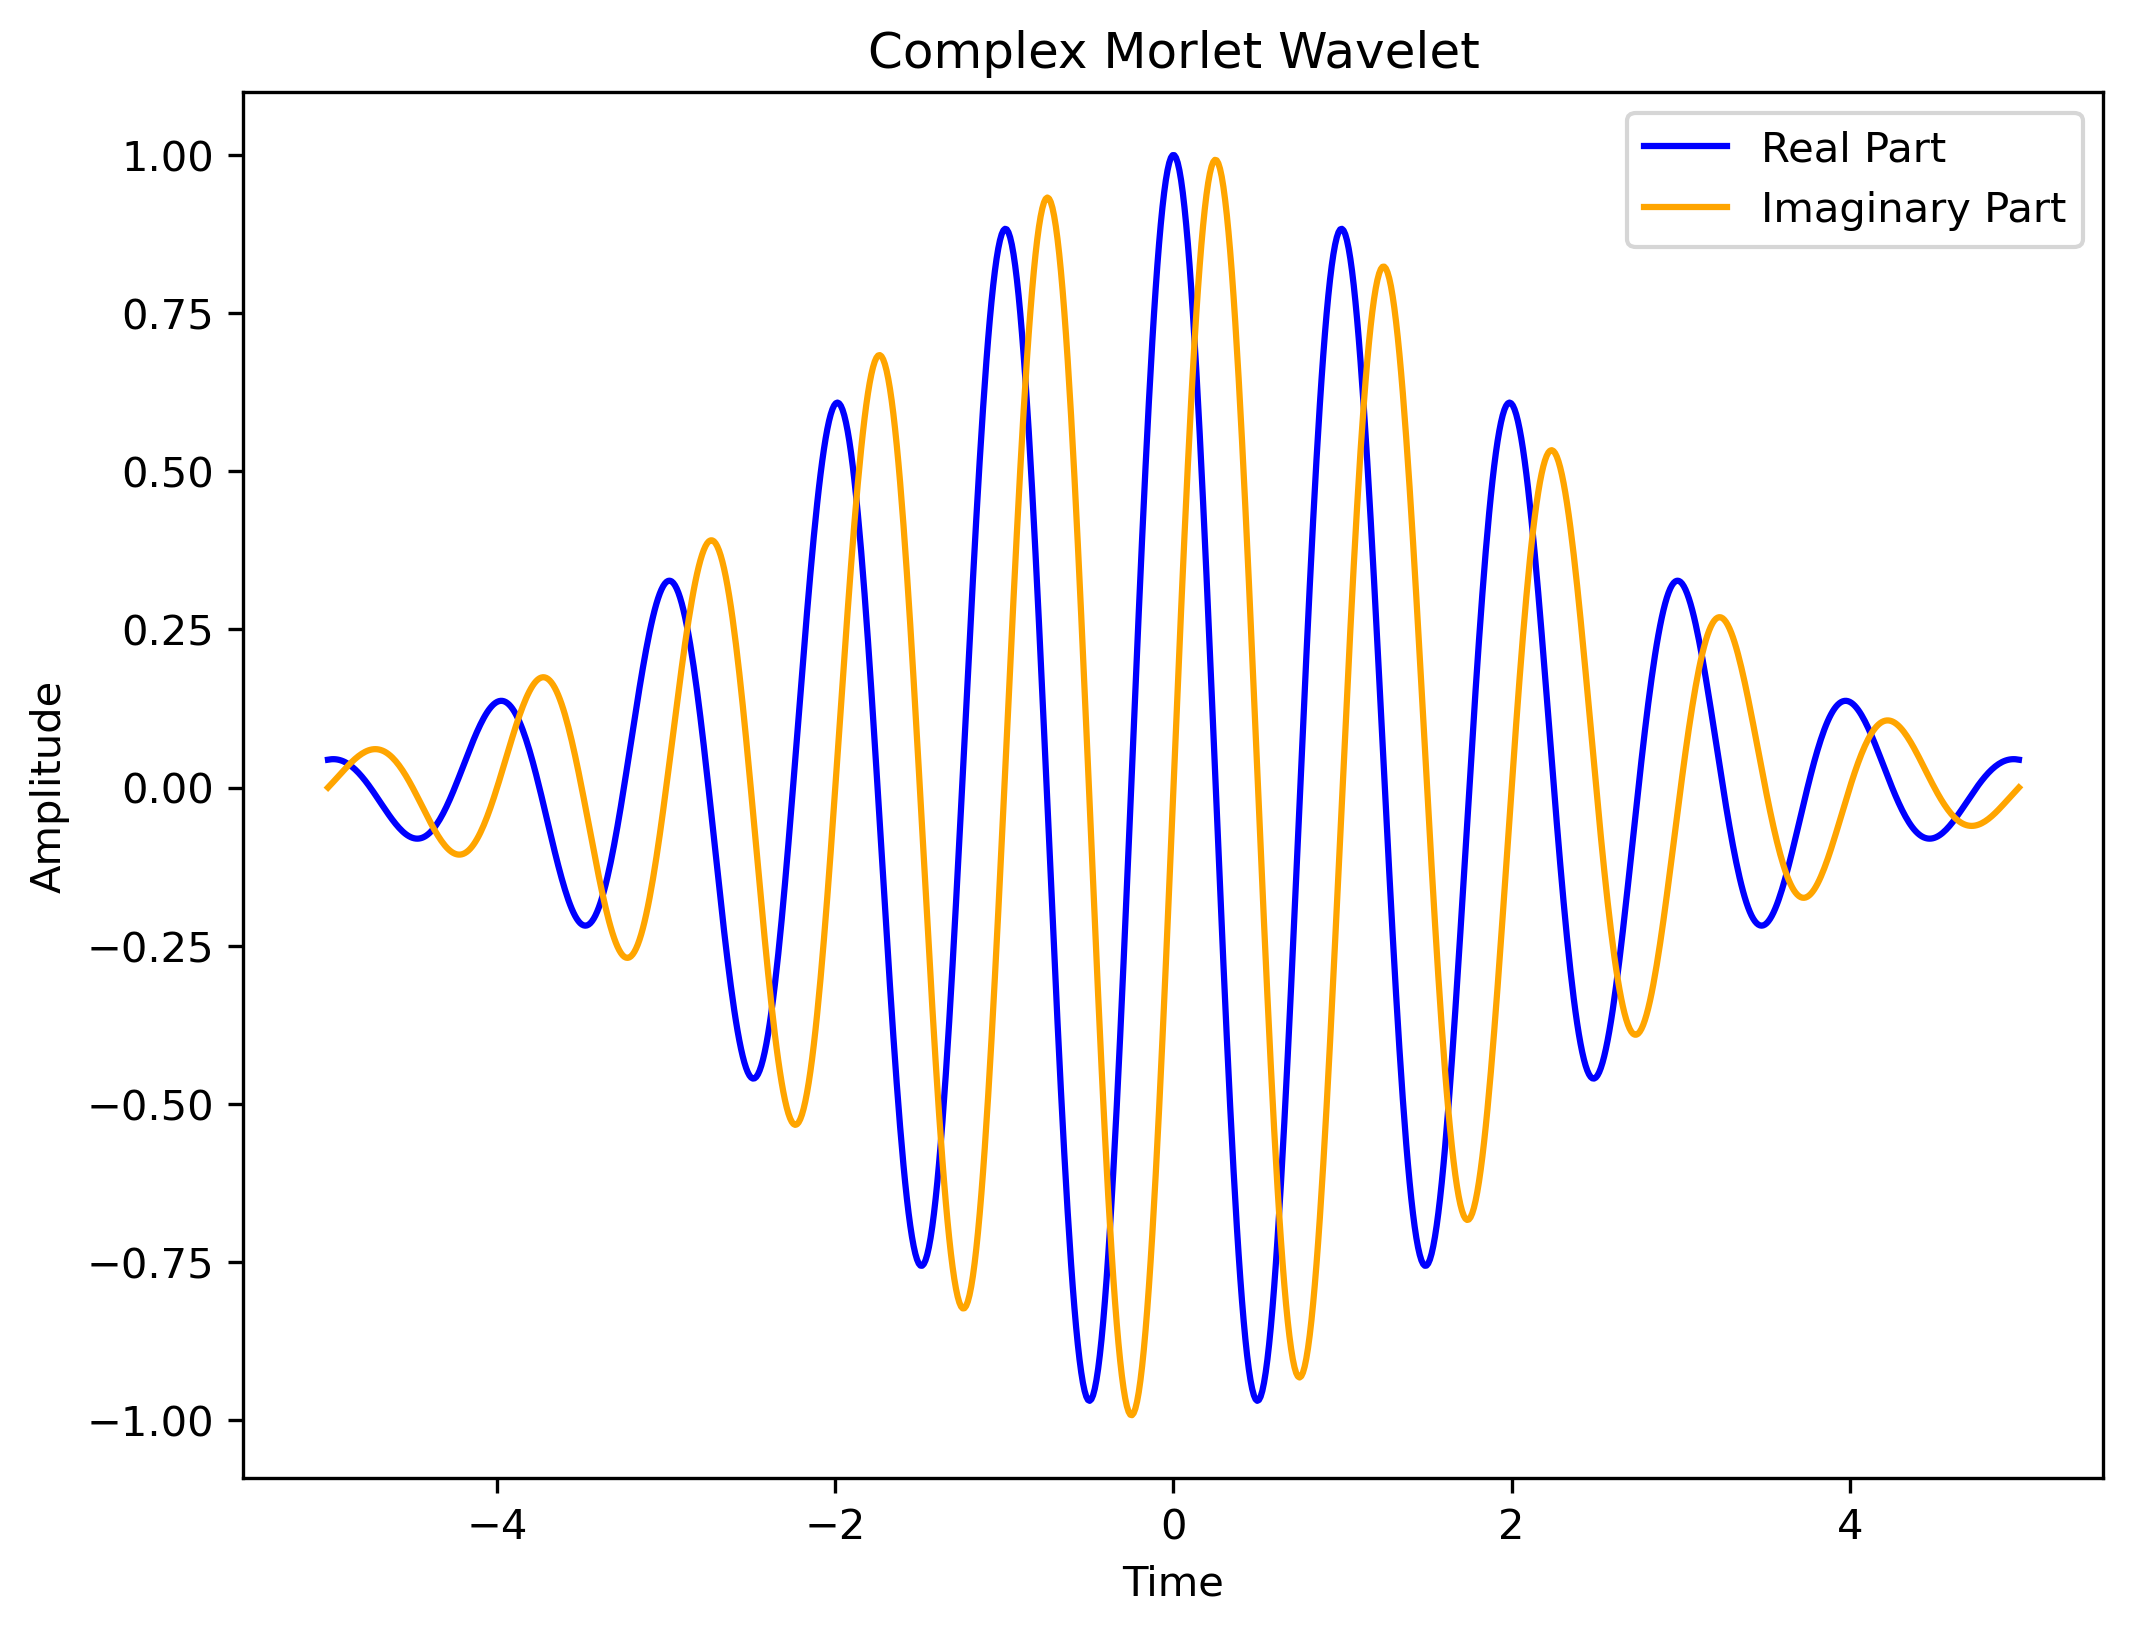
\includegraphics[width=\linewidth]{wavelet.png}
    \caption{The figure illustrates the real (blue) and imaginary (orange) components of a complex Morlet wavelet as a function of time. The wavelet exhibits oscillatory behavior that is localized in time, demonstrating its band-pass filtering characteristics. The central peak corresponds to the wavelet's maximum amplitude, representing the most significant contribution to the signal's frequency content. The symmetry and decay of the wavelet components reflect its Gaussian envelope, ensuring minimal leakage in time-frequency localization. }
    \label{fig:wavelet}
\end{figure}

Crucially, the selection of wavelet parameters significantly impacts the accuracy and interpretability of the analysis. The width of the Gaussian window, often parameterized as the number of cycles, governs the trade-off between temporal and spectral resolution. A smaller number of cycles enhances temporal precision but broadens the spectral response, whereas a higher number of cycles improves spectral resolution at the cost of temporal localization. Recent advancements propose defining wavelets in terms of full-width at half-maximum (FWHM) to provide more intuitive control over time and frequency smoothing \cite{cohen2019}. In general, optimal tailoring of wavelet parameters depends on the characteristics of the signal at hand and the purposes of the analysis.

There has been an abundance of research showcasing the efficacy of complex Morlet wavelets analysis in the biomedical field and especially in EEG analysis, but these findings can generalize to the analysis of LFP signals \cite{cohen2014}, as is the case here. Their ability to simultaneously preserve both temporal and spectral information has been extensively leveraged in many fields of neuroscience, such as traditional EEG analysis \cite{barlaam2018}, cognitive neuroscience \cite{perdomo2019}, affective neuroscience \cite{aruldass2022}, and the intersection of neuroscience and machine learning \cite{zhang2022}, thus indicating the versatility and efficaciousness of this particular representation in a diverse array of analyses.

\subsubsection{Autoregressive Modeling}

Autoregressive (AR) modeling is a fundamental technique in time-series analysis that captures temporal dependencies within data by expressing each observation as a linear function of its preceding values, with the addition of a stochastic noise component. This approach is particularly valuable in biomedical signal analysis, as it provides a compact and interpretable representation of time-series data such as Local Field Potential (LFP) recordings. By estimating the parameters of an AR model, one can extract meaningful features from LFP signals, which can then be used as inputs in machine learning classification tasks.

Mathematically, an autoregressive (AR) process of order \( p \) is defined as:

\[
X_t = \sum_{i=1}^{p} \phi_i X_{t-i} + \epsilon_t
\]

where:

\textcolor{green}{\( X_t \) is the current observation,
\( \phi_i \) are the autoregressive coefficients,
\( p \) is the model order,
\( \epsilon_t \) is a white noise term. \cite{box2008}}

The choice of \( p \) determines the complexity of the model and plays a crucial role in balancing overfitting and underfitting when representing time-series data. AR modeling serves as a powerful feature extraction technique, because instead of using raw time-series data, which may be high-dimensional and contain redundant or irrelevant information, the estimated AR coefficients provide a compact summary of the signal's temporal dynamics. This transformation facilitates training machine learning classifiers by reducing computational complexity and improving generalization.

Although for the purposes of this paper, a simpler model was implemented, it is worth noting that the foundational concept of Autoregressive modeling has been expanded into various forms, such as the Autoregressive Integrated Moving Average (ARIMA) model, which incorporates differencing to handle non-stationary data, and the Autoregressive Distributed Lag (ARDL) model, which allows for the inclusion of lagged independent variables alongside autoregressive terms \cite{agbenyega2022, natsiopoulos2022}.

While the convolution with complex morlet wavelets analyzes time-series in the time-frequency domain, AR models capture temporal dependencies without requiring a transformation into the frequency domain. Furthermore, AR analyses are significantly less resource-intensive and their results are easily interpretable. These \textcolor{green}{features make} autoregressive models particularly suitable for analyzing high-dimensional and volatile time series data, as seen in applications ranging from economic forecasting to biological systems \cite{regis2022}.

\subsubsection{N-Gram Graphs} \label{sec:graphs}

N-Gram Graphs is a method which was conceived in the context of Natural Language Processing (NLP) \cite{giannakopoulos2008, tsekouras2017}, as a summary evaluation method \cite{giannakopoulos2008summarization}, but its use has also been extended to other fields, such as the biomedical sciences \cite{kazantzidis2017, polychronopoulos2014}. Formally, an \( n \)-gram graph is defined as a directed or undirected graph 
\[
G = \{ V, E, W \}
\]
where:
\begin{itemize}
    \item \( V \) is the set of vertices representing distinct \( n \)-grams,
    \item \( E \) is the set of edges indicating co-occurrences of \( n \)-grams, and
    \item \( W \) is a function assigning weights to edges based on co-occurrence frequency.
\end{itemize}

An \( n \)-gram graph is created by fragmenting a sequence into overlapping segments of length \( n \), referred to as \( n \)-grams. These segments can be characters of text (also known as Q-grams \cite{ukkonen1992}) or words and they are considered to be in co-occurrence when they appear within a predefined window, which represents a maximum distance threshold between them. Within the graph representation, these \( n \)-grams serve as vertices, and their co-occurrence is depicted by edges connecting them. The weight of these edges can be assigned in various ways, with one of the most common methods being the frequency of co-occurrence within the specified window.

Character-based \( n \)-grams provide a finer level of detail compared to word-based counterparts, eliminating the necessity for explicit segmentation. The process of extracting \( n \)-grams involves sliding a window of length \( n \) across the sequence from the initial position, moving incrementally by one step at a time. This results in a total of 
\[
|s| - n + 1
\]
\( n \)-grams for a sequence of length \( |s| \). A smaller window size yields a greater number of \( n \)-grams but confines them to more localized neighborhoods. By incorporating multiple \( n \)-gram sizes within a specified range 
\[
[L_{\min}, L_{\max}]
\]
the \( n \)-gram graph effectively captures both macro-level and micro-level relationships within the sequence, enabling a more comprehensive representation of its structural properties \cite{gialitsis2023}.

Depending on the type of window used, different approaches for constructing the N-Gram graph can be applied.

In the \textbf{nonsymmetric approach}, a window of length \( n \) slides over the text, capturing only the preceding characters or words relative to \( N_0 \). If \( N_0 \) is positioned at \( p_0 \), then the window extends from \( p_0 - 1 \) to \( p_0 - n \), ensuring that only earlier occurrences are considered. The weight of each edge in this representation corresponds to the number of times two \( n \)-grams appear together within the window.

The \textbf{symmetric approach} differs in that the window is centered around the starting position of \( N_0 \). In this case, if \( N_0 \) is at \( p_0 \), the window spans from 
\[
p_0 - \lfloor n/2 \rfloor \quad \text{to} \quad p_0 + \lfloor n/2 \rfloor,
\]
incorporating both preceding and following characters or words. As with the nonsymmetric method, edges are weighted according to the frequency of co-occurrence of neighboring \( n \)-grams.

The \textbf{Gauss-normalized symmetric approach} extends the symmetric method by expanding the window size to \( 3 \times n \), centering it on \( N_0 \). If \( N_0 \) starts at \( p_0 \), the window extends from 
\[
p_0 - \lfloor 3n/2 \rfloor \quad \text{to} \quad p_0 + \lfloor 3n/2 \rfloor,
\]
thereby capturing a broader range of context. However, unlike the previous methods, this approach assigns edge weights based not only on co-occurrence frequency but also on the relative distance between the \( n \)-grams. Specifically, an \( n \)-gram \( N_1 \) at a distance \( d_1 \) from \( N_0 \) is assigned a lower influence than another \( n \)-gram \( N_2 \) at a closer distance \( d_2 \) (where \( d_2 < d_1 \)). \cite{giannakopoulos2008summarization}

This approach of representing a document as an n-gram graph is also used when representing a collection of documents associated with a particular topic, or as is the case here, a collection of time-series of particular classes. In this scenario, a consolidated class graph is constructed by integrating multiple individual document graphs (or time-series) through an update function. The process unfolds as follows: for a given set of documents assigned to topic $C_k$, an initially empty graph $G_{C_k}$ is established. Each document $d_m$ within the topic set is then converted into its corresponding document graph $G_{d_m}$, which is subsequently combined with $G_{C_k}$ to form an updated graph $G_u = (V_u, E_u, W_u)$. This updated graph is defined by:

\begin{align*}
    V_u &= V_{C_k} \cup V_{d_m}, \\
    E_u &= E_{C_k} \cup E_{d_m}, \\
    W_u(e) &= W_{C_k}(e) + (W_{d_m}(e) - W_{C_k}(e)) \times \frac{1}{m},
\end{align*}

where the vertex set $V_u$ and edge set $E_u$ are formed by the union of the corresponding elements from the class and document graphs. The weight function $W_u(e)$ adjusts iteratively, ensuring that edge weights gradually converge toward an averaged representation as more documents are integrated. This aggregation enables the class graph to encapsulate structural and contextual patterns characteristic of the entire topic.

\subsubsection{Similarity Measures for N-Gram Graphs} \label{sec:similarity_measures}

Several methods have been proposed in the literature for measuring the similarity between \( n \)-gram graphs. These functions evaluate different structural and weighted aspects of the graphs to determine their degree of correspondence. We will describe those that were used for the purposes of this thesis:

\paragraph{Size Similarity (SS)}

This measure quantifies the difference in the number of edges between two graphs. It penalizes discrepancies in graph size by computing the ratio of the smaller graph's edge count to the larger one's:

\[
SS(G_a, G_b) = \frac{\min(|G_a|, |G_b|)}{\max(|G_a|, |G_b|)}
\]

A similarity score closer to 1 suggests that both graphs have a comparable number of edges, whereas lower values indicate significant differences in structure.

\paragraph{Value Similarity (VSim)}

Value Similarity extends basic similarity measures by incorporating edge weights. For each matching edge \( e \), with weight \( W(e, G_x) \) in graph \( G_x \) and \( W(e, G_y) \) in graph \( G_y \), the contribution of that edge is determined by the Value Ratio (VR):

\[
VR(e) = \frac{\min(W(e, G_{a}), W(e, G_{b}))}{\max(W(e, G_{a}), W(e, G_{b}))}
\]

which is constrained to the range \([0,1]\). If an edge does not exist in both graphs, its contribution is zero. The overall Value Similarity is given by:

\[
VSim(G_{a}, G_{b}) = 
\frac{\sum_{e \in E_{a}} \frac{\min(W(e, G_{a}), W(e, G_{b}))}{\max(W(e, G_{a}), W(e, G_{b}))}}{\max(|E_{a}|, |E_{b}|)}
\]

This measure reaches its highest value of 1 when both graphs share identical edges with matching weights.

\paragraph{Normalized Value Similarity (NVSim)}

To account for discrepancies in graph size, Normalized Value Similarity (NVSim) modifies \( VSim \) by adjusting for the relative sizes of the compared graphs:

\[
NVSim(G_{a}, G_{b}) = 
\frac{\sum_{e \in E_{a}} \frac{\min(W(e, G_{a}), W(e, G_{b}))}{\max(W(e, G_{a}), W(e, G_{b}))}}{\min(|E_{a}|, |E_{b}|)}
\]

This normalization is particularly useful when one graph is significantly larger than the other, as it prevents the similarity score from being dominated by size disparities \cite{giannakopoulos2008, papadakis2016}. All the similarity measures described are symmetric and produce values within the interval \([0, 1]\), where a score of 1 indicates identical graphs, and 0 signifies completely dissimilar ones. When the \( n \)-gram length varies within a range \([L_{\min}, L_{\max}]\), similarity is computed separately for each rank. The final similarity score is then derived as a weighted sum of these individual scores, with the weights corresponding to the rank of each \( n \)-gram. This weighting scheme prioritizes higher-rank matches, as longer \( n \)-grams capture more detailed structural relationships and are thus considered more informative. \( VSim \) and \( NVSim \) consider the frequency of co-occurring \( n \)-grams, making them analogous to the cosine similarity applied to frequency-based vectors in bag-of-\( n \)-gram models. However, unlike traditional methods that evaluate the occurrence of individual \( n \)-grams, \( VSim \) and \( NVSim \) operate on pairs of \( n \)-grams, capturing their co-occurrence relationships.

\subsubsection{Classification with K - Nearest Neighbors algorithm} \label{sec:classification}

\textcolor{teal}{Before delving into the details of the $k$-Nearest Neighbors (k-NN) algorithm, it is important to briefly introduce the task of classification and the metrics used to evaluate it. In supervised classification, the goal is to assign data instances to predefined categories based on features extracted from labeled examples. The performance of classification models is typically assessed using a set of standard evaluation metrics, including accuracy, precision, recall, F1-score, sensitivity, and specificity. Each of these metrics captures a different aspect of model performance, such as overall correctness, balance between false positives and false negatives, or the ability to detect specific classes. These metrics \cite{sokolova2009} are formally defined as follows:}

Precision quantifies the correctness of positive predictions, defined as:

\[
\text{Precision} = \frac{\text{True Positives}}{\text{True Positives} + \text{False Positives}}
\]

Recall (or sensitivity) measures the ability of the classifier to identify all actual positive instances:

\[
\text{Recall} = \frac{\text{True Positives}}{\text{True Positives} + \text{False Negatives}}
\]

Specificity, in contrast, measures the ability to correctly identify negative instances:

\[
\text{Specificity} = \frac{\text{True Negatives}}{\text{True Negatives} + \text{False Positives}}
\]

The F1-score is the harmonic mean of precision and recall:

\[
\text{F1-score} = 2 \times \frac{\text{Precision} \times \text{Recall}}{\text{Precision} + \text{Recall}}
\]

The macro-averaged F1-score (\(\text{F1-macro}\)) is obtained by computing the F1-score for each class independently and then averaging the results:

\[
\text{F1-macro} = \frac{1}{N} \sum_{i=1}^{N} \text{F1-score}_i
\]

where \(N\) is the number of classes. This approach ensures that each class contributes equally to the final evaluation, regardless of class size, making it particularly informative when class distributions are imbalanced.

In this thesis, the evaluation metrics we used were Accuracy and the macro-averaged F1-score, as described in Chapter~\ref{sec:evaluation}, which provide a comprehensive assessment of model performance, while ensuring that factors such as class imbalance are taken into consideration.

The K-Nearest Neighbors (KNN) algorithm is a widely utilized machine learning technique that is particularly suitable for classification and regression tasks. As a non-parametric, meaning it doesn't make assumptions about the structure of the data, instance-based learning algorithm, KNN operates on the principle of similarity, assuming that data points with close proximity in the feature space belong to the same class. Its simplicity and effectiveness have made it one of the foundational approaches in pattern recognition and classification problems.

KNN is an instance-based learning algorithm, meaning that it does not construct an explicit generalization model during a training phase. Instead, it retains the entirety of the training data and makes predictions by comparing new input data to the stored instances. This approach, often referred to as lazy learning, contrasts with parametric methods such as linear regression or support vector machines, where a model is explicitly trained before making predictions \cite{gavagsaz2022}. At its core, this method operates by calculating the distance between the target data point and all other points in the training dataset, typically using metrics such as Euclidean distance \cite{sinulingga2023}.

The classification process in KNN follows a straightforward approach: for a given test instance, the algorithm identifies the \( K \) closest data points from the training set and assigns the majority class among those neighbors to the test instance. The choice of \( K \) plays a critical role in balancing variance and bias in classification performance. Small values of \( K \) make the classifier more sensitive to noise, whereas larger values may lead to excessive smoothing and misclassification of boundary points.

\paragraph{Distance Metrics in KNN} A key aspect of KNN's effectiveness is the choice of distance metric, which quantifies the similarity between data points. Several distance measures have been proposed in the literature, with the most commonly used being Euclidean distance, Manhattan distance, Minkowski distance, and Cosine similarity \cite{leskovec2020}. The selection of an appropriate metric is particularly relevant in LFP-based classification tasks, as different representations of the data may influence classification accuracy, as was shown in a paper on sentiment classification tasks \cite{romli2021}.

\paragraph{Euclidean Distance:}
The Euclidean distance is the most widely used metric and is defined as
\[
d(x, y) = \sqrt{\sum_{i=1}^n (x_i - y_i)^2}
\]

where \( x \) and \( y \) are two points in an \( n \)-dimensional space. This metric assumes that all features contribute equally to the similarity computation.

\paragraph{Manhattan Distance:}
Manhattan distance, also known as taxicab distance, is defined as:

\[
d(x, y) = \sum_{i=1}^n |x_i - y_i|
\]

Unlike Euclidean distance, Manhattan distance considers the absolute differences between feature values, making it more robust to high-dimensional spaces where sparse features are present.

\paragraph{Minkowski Distance:}
Minkowski distance generalizes both Euclidean and Manhattan distances and is defined as:

\[
d(x, y) = \left( \sum_{i=1}^n |x_i - y_i|^p \right)^{\frac{1}{p}}
\]

where \( p = 2 \) reduces to Euclidean distance, and \( p = 1 \) corresponds to Manhattan distance. The Minkowski parameter \( p \) allows for greater flexibility in adjusting the sensitivity of distance calculations.

\paragraph{Cosine Similarity}

For high-dimensional feature spaces, cosine similarity is an effective measure of similarity:

\[
\cos(x, y) = \frac{x \cdot y}{\|x\| \|y\|}
\]

where \( x \) and \( y \) are vectors. Cosine similarity evaluates the angular distance between vectors rather than their absolute difference.

The selection of the optimal parameter set and distance metric can be achieved through heuristic techniques and close inspection of the data. It is worth noting, that KNN algorithms while effective, also come with limitations, such as sensitivity to noise and the curse of dimensionality, which can degrade performance in high-dimensional spaces \cite{ding2017, triguero2019}.

\section{Related Work}
When researching the literature regarding the use of the aforementioned representations of data for machine learning tasks in the context of epilepsy, one comes across many studies focusing primarily on EEG signals. As mentioned earlier the basic concepts and principles remain unchanged whether we focus on EEG, LFP or ECoG signals.

One such example is a study by Singh and Dehuri (2020) \cite{singh2020}, which addresses the challenge of automatic epileptic seizure detection using electroencephalogram (EEG) signals. The complexity arises from the non-linear and non-stationary nature of EEG signals, which makes their analysis in the time domain particularly difficult. The researchers propose a novel classification approach that combines discrete wavelet transform (DWT) for feature extraction, singular value decomposition (SVD) for eigenspace analysis, and a fuzzy k-nearest neighbor (FkNN) classifier to categorize EEG signals into five different classes.

To evaluate the efficacy of their approach, they used the publicly available Bonn University EEG dataset, which contains EEG recordings from both healthy individuals and epileptic patients in different states. They tested their method on two-class, three-class, and five-class classification tasks. Their experimental results indicate that the proposed DWT-SVD-FkNN model achieves 100\% accuracy in two-class and three-class classifications and 93.33\% accuracy in the more complex five-class classification. Statistical validation using ANOVA confirmed the significance of the extracted features.

The study's findings demonstrate that the proposed method outperformed several existing classification techniques in terms of accuracy and computational speed. As future directions, the authors suggested applying their approach to larger EEG datasets and exploring alternative feature extraction methods, such as variational mode decomposition (VMD), to enhance classification performance. They also proposed incorporating additional statistical measures, such as different entropy types and power spectral density, to further refine their model.

Similarly, Mardini et al. (2020) \cite{mardini2020} addressed the challenge of epileptic seizure detection from EEG signals using machine learning classifiers. The primary problem they tackled was the need for an accurate and computationally efficient method to differentiate between normal and epileptic EEG signals, bypassing the need for manual expert analysis, which is time-consuming and prone to errors. Their aim was to improve classification accuracy while reducing computational costs by leveraging advanced feature selection techniques and multiple classifiers.

To achieve this, they proposed a framework that extracts features from EEG signals using 54 discrete wavelet transform (DWT) mother wavelets. These extracted features were then optimized using a genetic algorithm (GA) to select the most relevant features for classification. The selected features were fed into four different machine learning classifiers: Support Vector Machine (SVM), k-Nearest Neighbors (KNN), Artificial Neural Network (ANN), and Naïve Bayes (NB). The framework was tested on 14 different two-class epilepsy detection scenarios, using EEG data from the same Bonn University dataset.

The evaluation of their model was done using three key performance metrics: accuracy, sensitivity, and specificity. The results indicated that all four classifiers performed competitively, but ANN consistently achieved the highest accuracy, outperforming the other classifiers across most dataset combinations. In some cases, accuracy reached 100\%, while in others, it ranged between 93.3\% and 98.8\%. Sensitivity and specificity also showed strong results, with ANN achieving the best average values.

Based on above findings, the conclusion was that the proposed DWT-GA-ANN approach significantly improves epilepsy detection. The authors recommended further exploration of deep learning models, such as state-of-the-art neural networks, to enhance classification performance. Additionally, they suggested applying their methodology to different EEG datasets from diverse populations to test the generalizability of their model.

Furthermore, this \cite{sharmila2016} study by Sharmila and Geethanjali focuses on enhancing epileptic seizure detection from EEG signals using machine learning classifiers and specifically, an automatic classification framework that leverages discrete wavelet transform (DWT) for feature extraction and employs both naïve Bayes (NB) and k-nearest neighbor (k-NN) classifiers to detect seizures.

In this case, the method involved decomposing EEG signals using DWT into different frequency bands and extracting statistical features such as mean absolute value (MAV), standard deviation (SD), and average power (AVP) from specific sub-bands. These extracted features served as inputs to the classifiers. The study evaluated the classification performance using fourteen different two-class combinations, where seizure data (Set E) was compared with different normal and interictal states (Sets A–D).

The researchers assessed the effectiveness of their method using accuracy, sensitivity, and specificity metrics. Their results demonstrated that the NB classifier consistently outperformed k-NN in most cases, achieving an accuracy of 100\% for certain combinations, particularly for normal eyes-open (Set A) versus seizure (Set E). The k-NN classifier performed comparably well, achieving 100\% accuracy in some cases, but generally exhibits slightly lower classification accuracy than NB. Additionally, NB is found to be computationally more efficient, making it more suitable for real-time seizure detection applications.

The authors recommended using the NB classifier for epileptic seizure detection due to its superior accuracy and lower computational cost. They suggested that future research should explore additional statistical features, integrate other classification techniques, and apply their method to larger EEG datasets to further validate and enhance its reliability.

Gajic et al. (2014) \cite{gajic2014} also tackled the challenge of detecting epileptic seizures from EEG signals using an automated classification system based on wavelet transform and statistical pattern recognition. The study aimed to develop a reliable, automated system that can distinguish between normal, interictal (seizure-free), and ictal (seizure) EEG signals, thereby improving epilepsy diagnosis and patient monitoring.

The researchers proposed a three-stage classification pipeline: (1) feature extraction using wavelet transform, (2) dimensionality reduction using scatter matrices, and (3) classification using quadratic classifiers. The EEG data was decomposed into clinically relevant frequency sub-bands (delta, theta, alpha, beta, and gamma), and statistical features such as energy, entropy, and standard deviation were extracted. The feature space was then reduced to enhance classification accuracy and efficiency before being input into quadratic classifiers that categorized EEG signals into one of the three groups.

The results demonstrated that the system achieves an overall classification accuracy of 99\%, with 100\% accuracy for normal EEG, and 98\% accuracy for both interictal and ictal EEG signals. These findings confirmed the robustness of the proposed algorithm in classifying EEG signals and detecting epileptic seizures.

Finally, this study \cite{golfidis2023} by Gkolfidis et al. (2023) coming from our lab, set out to find the optimal solution for classifying different epileptic activity states—endogenous (preictal), interictal, and seizure-like (ictal)—from local field potential (LFP) recordings in mice. To achieve this, the researchers recorded LFP signals from layers II/III of the primary somatosensory cortex of young mice and applied the Highly Comparative Time Series Analysis (HCTSA) toolbox to extract over 4000 features from the signals. These features were derived from time, frequency, time-frequency, and chaotic domains, obtained after performing over 7700 time-series analysis operations. The dimensionality of the feature space was reduced using a combination of correlation analysis and random-forest recursive feature elimination with cross-validation (RF-RFECV), resulting in a reduced set of 22 features for distinguishing endogenous from interictal activity and 27 features for distinguishing interictal from seizure-like activity.

The researchers tested nine ML classifiers, including linear and polynomial support vector machines (SVMs), a radial basis function (RBF) SVM, random forest (RF), decision trees (DT), and k-nearest neighbors (kNN). Their results indicated that the RBF SVM achieved the best performance, with a Cohen kappa score of 0.9914 for endogenous vs. interictal classification using just 22 features, and 0.9565 for interictal vs. seizure-like classification using 27 features. These findings suggested that ML-based analysis of cortical LFP signals can provide highly accurate seizure detection and prediction, confirming that the proposed ML-based pipeline holds significant potential for improving seizure detection and prediction in focal epilepsy.

\textcolor{red}{Collectively, these studies demonstrate the potential of various data representations—particularly wavelet-based and statistical methods—for effective classification of epileptic states, primarily using EEG data. However, they have not addressed the characterization and classification of quiescent segments specifically within LFP signals during different stages of epileptogenesis. This gap is significant, as these segments may carry crucial information about the underlying neural dynamics leading to seizure onset. Therefore, the present thesis aims to explore and compare different representations of LFP data—wavelet convolution, autoregressive modeling, and n-gram graphs—for their effectiveness in classifying quiescent segments across distinct epileptic states, with the broader goal of improving our understanding of these subtle yet potentially informative periods of neuronal activity.
}

\section{Materials and Methods}
\subsection{Data Collection}
Data were obtained from this study \cite{vasilopoulos2023} by Vasilopoulos et al. as part of the electrophysiology lab spearheaded by Professor Irini Skaliora, PhD, at the Biomedical Research Foundation (BRFAA) of the Academy of Athens. All experiments were conducted in accordance with institutional and national guidelines for the ethical treatment of animals and were approved by the relevant ethical review boards. Male and female mice were used for all experiments between postnatal days 5 and 20 (P5--P20). Mice were weaned at postnatal day 21 and housed in groups of 5--7 in cages (267 mm $\times$ 483 mm $\times$ 203 mm) with bedding material under controlled environmental conditions (temperature: 21--24$^{\circ}$C, humidity: 50--60\%, ventilation: 10--12 air changes/hour, 12-hour light/dark cycle). Food and water were available \textit{ad libitum}.

The transgenic mouse model used in this study was indistinguishable from its Wild-Type counterpart. Acute brain slices were prepared by anesthetizing and rapidly decapitating the mice, and their brains were extracted and placed immediately in ice-cold oxygenated (95\% O$_2$--5\% CO$_2$) dissection buffer containing (in mM): 200 sucrose, 10 glucose, 26 NaHCO$_3$, 3.5 KCl, 1.2 NaH$_2$PO$_4$, 1 MgSO$_4$, 2 CaCl$_2$ (pH 7.4; 298 $\pm$ 5 mOsm).

Coronal brain slices (400 $\mu$m thick) were obtained using a vibratome (Leica VT1000S) and transferred to a holding chamber containing artificial cerebrospinal fluid (ACSF) at room temperature (24--26$^{\circ}$C) for at least one hour before recording. ACSF was composed of (in mM): 126 NaCl, 3.5 KCl, 26 NaHCO$_3$, 1.2 NaH$_2$PO$_4$, 1 MgSO$_4$, 2 CaCl$_2$, and 10 glucose (pH 7.4; 317 $\pm$ 4 mOsm). Slices were continuously oxygenated (95\% O$_2$--5\% CO$_2$) to maintain metabolic viability.

Following the recovery period, slices were transferred to a submerged-type recording chamber that allowed up to four slices to be recorded simultaneously under identical conditions. Slices were continuously perfused with oxygenated ACSF at a flow rate of 10--15 ml/min using a vacuum pump to ensure optimal oxygenation of the tissue.

Local field potential (LFP) recordings were obtained from layers II/III of the primary somatosensory cortex using low-impedance ($\sim$0.5 M$\Omega$) glass micropipettes filled with ACSF. Recording pipettes were made from borosilicate glass (1.5 mm outer diameter, 0.86 mm inner diameter, with inner filament) and pulled using a P-97 micropipette puller (Sutter Instrument Co., Novato, CA, USA). LFP recordings were performed in current-clamp mode using a Multiclamp 700B amplifier (Molecular Devices, San Jose, CA, USA). Signals were low-pass filtered at 6 kHz and digitized at 15 kHz using a 16-bit multi-channel interface (InstruTECH ITC-18, HEKA Elektronic, Germany).

After recording spontaneous cortical activity in normal ACSF for 20 minutes, the perfusion temperature was increased to 32--35$^{\circ}$C to induce epileptiform activity using one of two distinct \textcolor{red}{\textit{in vitro} models}:

\begin{itemize}
    \item \textbf{Low-Magnesium Model:} \textcolor{red}{Mg$^{2+}$-free ACSF was used}, removing the voltage-dependent block of NMDA receptors and leading to a hyperexcitable network state.
    \item \textbf{4-Aminopyridine (4-AP) Model:} 100 $\mu$M 4-AP (Sigma-Aldrich, St. Louis, MO, USA) was added to the ACSF to block voltage-gated potassium channels, thereby enhancing interneuron excitability and promoting seizure-like events.
\end{itemize}

Slices were continuously perfused in the pro-epileptic conditions for up to 80 minutes to allow for stabilization of epileptiform discharges. In this thesis, \textbf{only data obtained from the Low-Magnesium model were used}.

LFP recordings were analyzed using custom MATLAB scripts and the LFPAnalyzer software package \cite{kaplanian2022, tsakanikas2017}. The analysis pipeline included the preprocessing of the data, whereby LFP signals were DC offset-corrected and low-pass filtered at 200 Hz, the detection of Up and Down States (spontaneous network activity) using a combination of Hilbert transform and short-term energy methods, the analysis of the signals into their frequency components using Fourier transforms with a Kaiser window function to minimize spectral leakage, the extraction of the Entire Spiking Activity (ESA) using band-pass filtering (300--4000 Hz) followed by full-wave rectification and low-pass filtering at 100 Hz and the detection of Seizure-like events, which were defined by a tonic high-frequency burst followed by clonic afterdischarges, with transitions marked by spreading depolarizations (large DC shifts).

\subsection{Extraction of Down-states/Quiescent periods}
Out of all the data produced as part of the aforementioned study by Vasilopoulos et al., we made use of nine recording sessions. Each recording session consists of five or six recordings with a duration of 20 minutes each, which were saved as .mat files. The sampling frequency is 15.385 Hz. The activity observed in these recordings can be categorized in distinct states. 

The first recording in each recording session corresponds to the endogenous cortical activity, characterized by the distinctive appearance of Up and Down states (UDs), before any experimental intervention. 

At the start of the second recording, the 0 Mg$^{2+}$ model is initiated, marking the onset of the transitional phase, which typically lasts until the end of the second or third recording. This phase is further subdivided into two states: transitional pre-Spreading Depolarization (pre-SD) and transitional post-Spreading Depolarization (post-SD). The transition between these states is described in detail  in Section~\ref{sec:spreading_depolarization}.

The fourth and final phase, termed the ictal phase, begins with the appearance of Seizure-like Events (SLEs) and continues until the end of the final recording in the session. 

To summarize, the phases of neuronal activity in the context of induced epileptic activity can be divided as follows:
\begin{itemize}
    \item \textbf{Endogenous Activity} (or simply "EA")
    \item \textbf{Transitional pre-SD Activity} ("pre-SD")
    \item \textbf{Transitional post-SD Activity} ("post-SD")
    \item \textbf{Ictal Activity} 
\end{itemize}
Each of these phases includes periods of quiescence, where no event is observed. In the endogenous phase, quiescence appears in the form of Down states, whereas in the pre-SD, post-SD, and ictal phases, it occurs before or after Seizure-like Events or other events in the transitional period. As mentioned in the Introduction, we refer to these segments collectively as \textbf{quiescent segments}. 

We extracted quiescent segments using Matlab ver. R2024a (The MathWorks Inc., Natick, MA, United States) in conjunction with LFPAnalyzer, which automatically identifies and flags the starting and ending point of events in the LFP signal. These events were also confirmed by a specialist. This process resulted in a dataset of 598 quiescent segments, distributed as follows: 
\begin{itemize}
    \item \textbf{EA class}: 210 segments
    \item \textbf{Pre-SD class}: 128 segments
    \item \textbf{Post-SD class}: 138 segments
    \item \textbf{Ictal class}: 122 segments
\end{itemize}
Each instance within these classes varies in duration, with the minimum and maximum time spans differing significantly across categories.

The \textcolor{red}{endogenous activity class} exhibits instance durations ranging from approximately 0.99 seconds to 113.19 seconds. The pre-SD class presents durations from 1.07 seconds to 373.81 seconds, while the post-SD category demonstrates the most extensive variation, with instances lasting between 1.05 seconds and 585.79 seconds. Finally, the ictal class displays a range spanning from 1.53 seconds to 258.21 seconds.

In addition to temporal characteristics, the descriptive statistics of the amplitude of the quiescent segments for each class are as follows: The mean amplitude for the endogenous class is $-1.51 \times 10^{-8}$, with a standard deviation of $2.00 \times 10^{-6}$. The transitional pre-SD class presents the lowest mean amplitude at $-1.21 \times 10^{-7}$, with a standard deviation of $2.00 \times 10^{-6}$, while the transitional post-SD class is characterized by a mean amplitude of $-6.32 \times 10^{-8}$ and a standard deviation of $3.00 \times 10^{-6}$. Finally, the ictal class exhibits a mean amplitude of $2.63 \times 10^{-8}$ and a standard deviation of $3.00 \times 10^{-6}$. 

\textcolor{red}{To assess whether the distributions of mean amplitudes differed significantly across the four experimental classes (EA, Pre-SD, Post-SD, and Ictal), a sequence of statistical tests was conducted. First, the assumption of normality was tested within each class using the Shapiro-Wilk test. All classes exhibited significant deviations from normality (all $p < 10^{-13}$), indicating non-Gaussian distributions. Additionally, Levene's test revealed a significant difference in variances across groups ($p = 8.03 \times 10^{-11}$), violating the assumption of homogeneity of variances. Based on these results, the non-parametric Kruskal-Wallis H-test was employed as an alternative to one-way ANOVA. The test yielded a statistically significant difference in mean amplitudes across the classes ($H = 29.91$, $p = 1.44 \times 10^{-6}$), warranting post-hoc analysis. Dunn’s test with Holm correction for multiple comparisons was subsequently applied. The results indicated that the Ictal class differed significantly from all other classes (all $p < 0.01$), whereas no significant differences were observed between the EA, Pre-SD, and Post-SD classes. These findings suggest that the Ictal class exhibits a distinct amplitude profile, which may reflect unique underlying neural dynamics relative to non-ictal conditions.}

\subsection{Implementing N-Gram Graphs}
To implement the N-Gram Graphs representation, we followed a structured procedure. First, each time series (instance) in the dataset was transformed into a symbolic sequence. This was achieved by discretizing the y-axis using the \texttt{KBinsDiscretizer} from \texttt{scikit-learn}~\cite{scikit-learn}, assigning a unique symbol to each bin. The x-axis of each time series was then segmented into equal-length chunks, and the mean value of each chunk was computed. Each chunk was subsequently assigned the symbol corresponding to the bin in which its mean value fell, resulting in a symbolic representation of the original time series (see Figure~\ref{fig:binning}).

\textcolor{green}{Once the symbolic sequences were generated, an n-gram graph was constructed for each instance. To obtain a representative graph for each class (control, pre-SD, post-SD, and ictal), we randomly selected 90\% of the graphs within each class and aggregated them. This proportion was chosen to ensure a robust and generalizable representation of the class while avoiding overfitting to the entire class data. The selection was independent of model training and cross-validation and aimed solely at building stable, representative graphs. In total, four representative graphs were generated—one for each class.}

Each instance in our dataset was then compared to these representative graphs using the similarity metrics presented in section~\ref{sec:similarity_measures}, namely:
\begin{itemize}
    \item \textbf{Size Similarity (SS)}
    \item \textbf{Value Similarity (VSim)}
    \item \textbf{Normalized Value Similarity (NVSim)}. 
\end{itemize}    
This process yielded \textbf{12 values} per instance \textbf{(4 representative graphs × 3 similarity metrics)}, which constitute the n-gram graph representation. The graphs were constructed by implementing the \textbf{nonsymmetric approach} (see Section~\ref{sec:graphs}), \textcolor{green}{which captures only preceding co-occurrences of $n$-grams relative to a reference position. This design introduces an inherent directionality in the graph, as edges reflect a temporal or sequential ordering—i.e., which $n$-grams precede others—rather than symmetric mutual co-occurrence. Directionality is crucial in this context because it preserves the causal or temporal flow of patterns in the time-series data, which may be informative for distinguishing between different classes of neural activity.}

\begin{figure}[htbp]
    \centering
    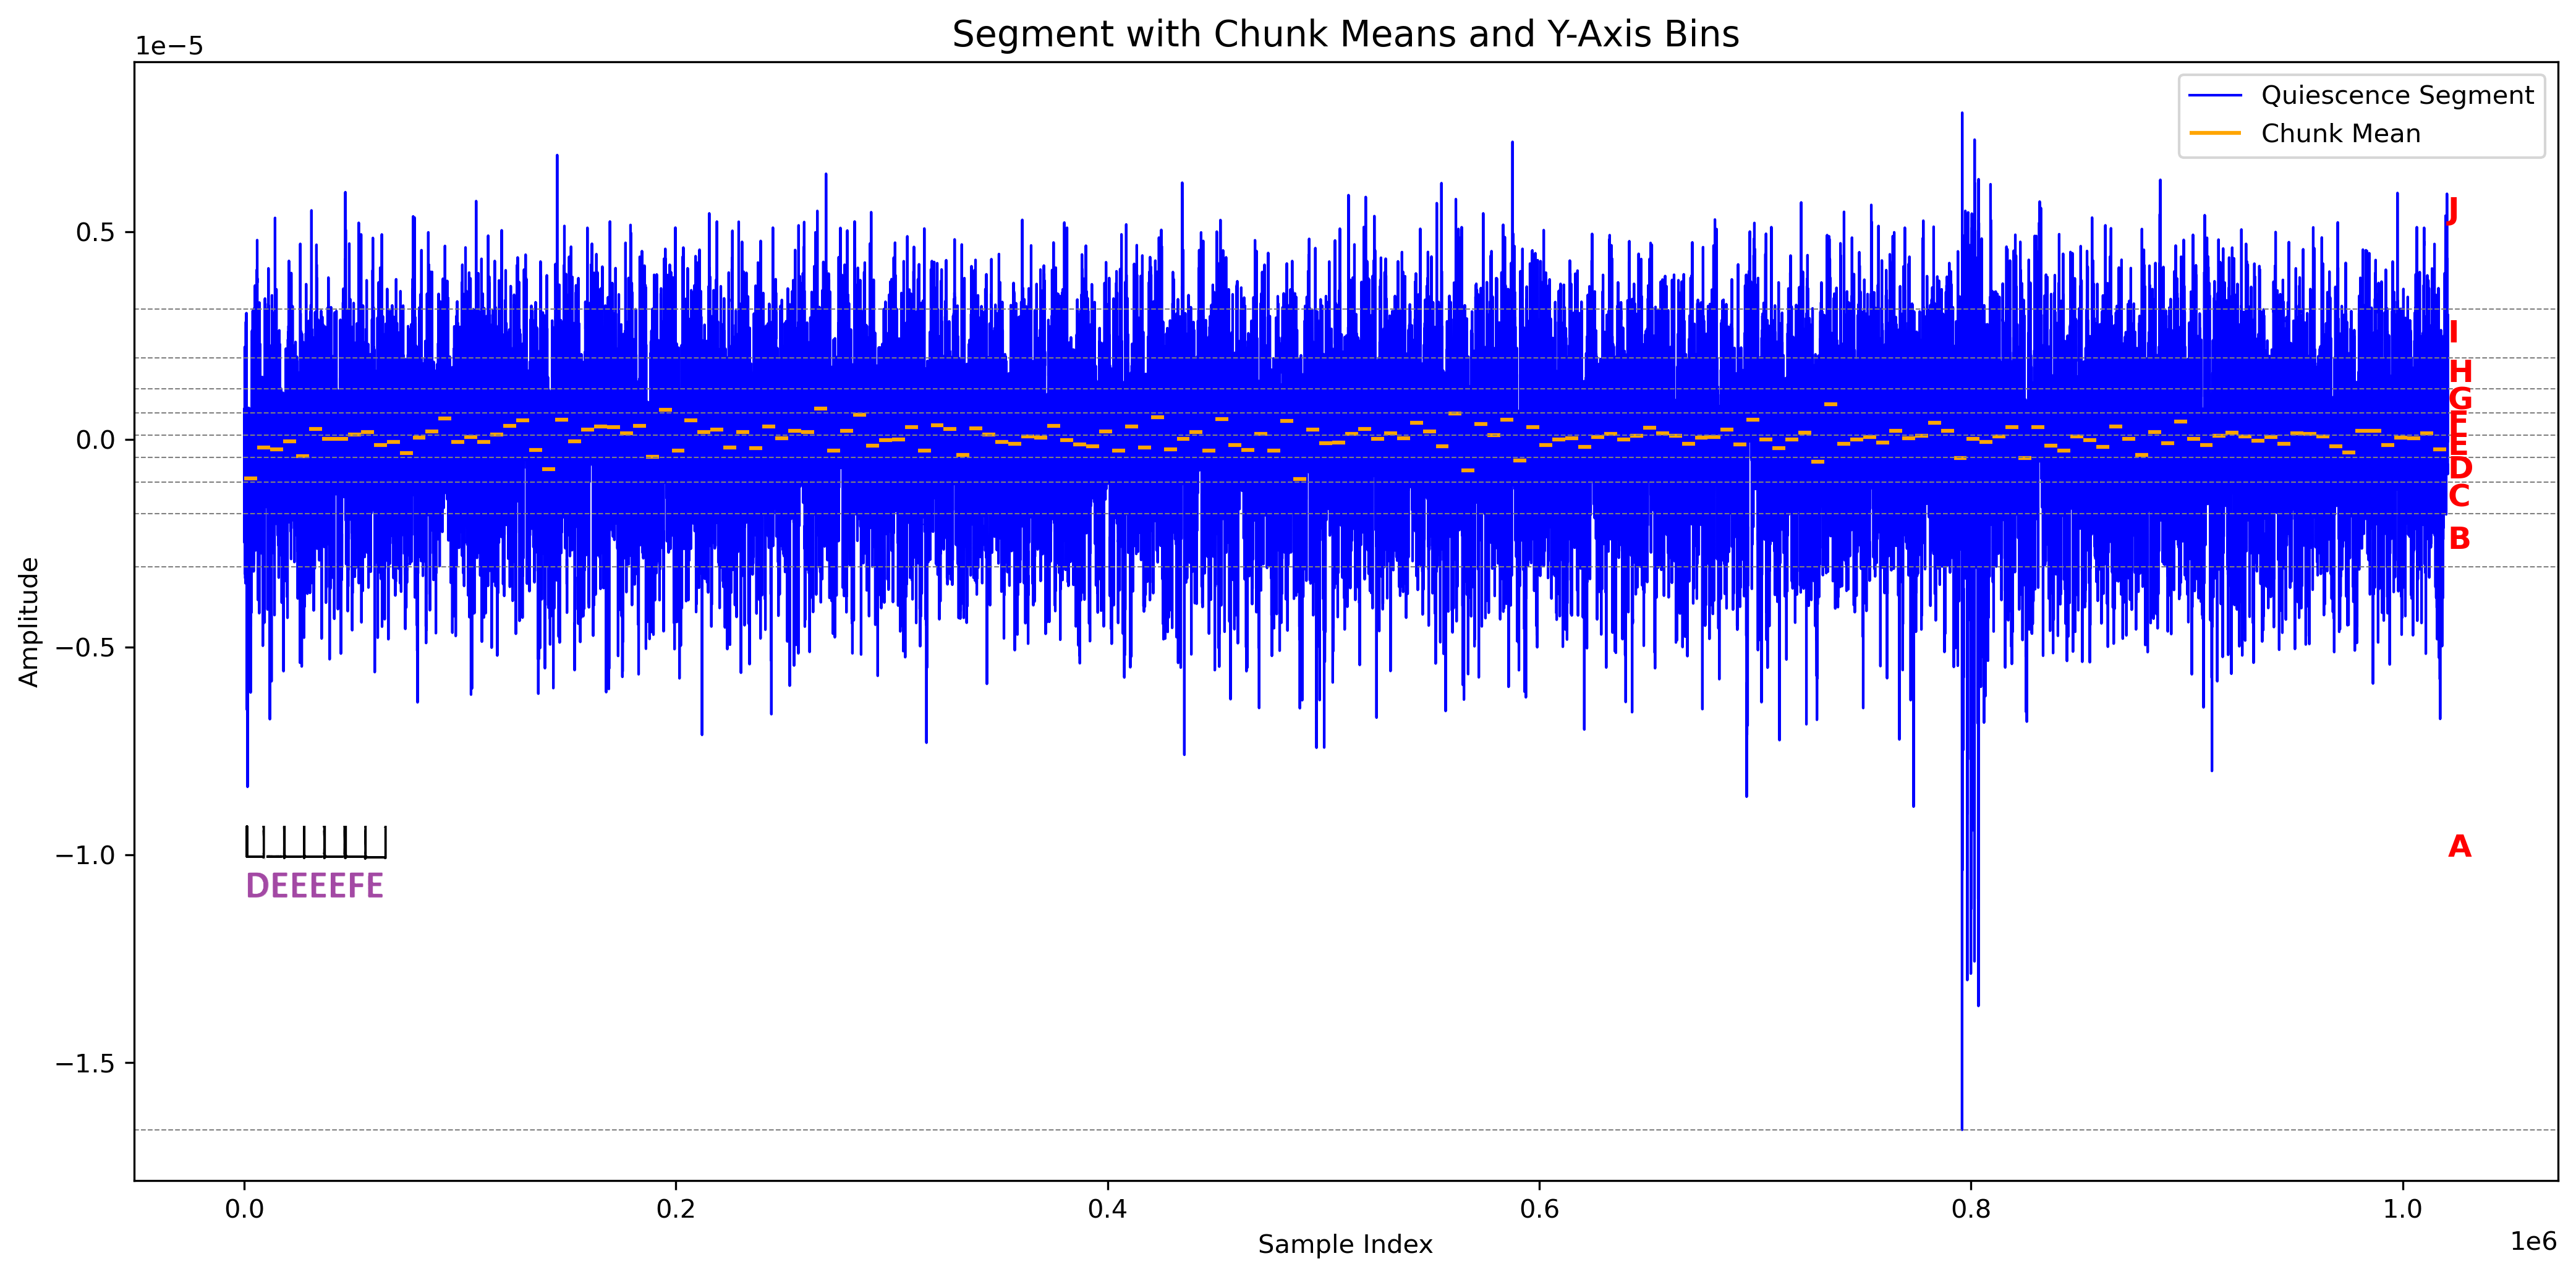
\includegraphics[width=\linewidth]{graph_binning_with_chunks_high_res1_ready.png}
    \caption{Conversion of a time series into a symbol series. The y-axis is divided into bins, indicated by dotted lines, with each bin assigned a corresponding letter (shown in red). \textcolor{green}{To ensure an approximately equal number of values in each bin, the binning was performed using the \texttt{KBinsDiscretizer} from \texttt{scikit-learn} with the \texttt{strategy='quantile'} parameter.} The x-axis is partitioned into chunks, displayed at the bottom of the figure, with each chunk labeled according to the bin in which its mean value falls (letters shown in purple). Only a portion of the purple labels is displayed here to indicate that the transformation process continues.}
    \label{fig:binning}
\end{figure}

\subsection{Parameter Selection}

\textcolor{green}{To identify optimal parameter configurations for each representation method explored in this study, an exploratory evaluation framework was employed. For each representation -Convolution with Complex Morlet Wavelets, Autoregressive Modeling and N-Gram Graphs- a range of parameter combinations was systematically tested, and their performance was assessed using stratified cross-validation to ensure robustness and mitigate the risk of overfitting. The evaluation metrics accuracy and macro-averaged F1 score were averaged across folds and compared to determine the most effective configurations. One-way ANOVA was used to support this comparison, with the primary goal of identifying practical, high-performing configurations under realistic data constraints. It is important to note that for this initial stage of parameter selection, the assumptions of normality and homogeneity of variances were not explicitly tested and a non-parametric test could have been more appropriate, but due to time constraints, reanalysis was not feasible. However, the selected parameters still reflect empirically observed performance trends across multiple folds and configurations, providing a well-informed foundation for the subsequent classification experiments.}
	
Specifically, for the wavelet convolution \textcolor{green}{exploratory frequency analysis was carried out to inform the selection of relevant frequency bands. The Fast Fourier Transform (FFT) was computed and plotted for a random subset of quiescent signal segments from each class. The visual inspection aimed to identify frequency bands that consistently exhibited elevated power relative to the rest of the spectrum. Although no strict power threshold was applied, this qualitative analysis revealed that the most prominent components typically fall within the delta (1–4 Hz), theta (4–8 Hz), alpha (8–13 Hz), beta (13–30 Hz), and, in some cases, the gamma (30–100 Hz) ranges. The selection of these bands was thus empirically guided by the observed spectral characteristics of the data, in alignment with conventional neurophysiological frequency definitions. Furthermore, we tested different combinations of target frequencies and wavelet design parameters. Specifically, three sets of target frequencies (in Hz) were evaluated: \{2, 4, 6, 8, 10, 15\}, \{2, 5, 10, 20, 40, 60\}, and \{5, 15, 30, 50, 70, 100\}. These frequencies represent the specific components of the signal we aim to extract using the wavelet transform.}

\textcolor{green}{In addition to the choice of target frequencies, we varied two intrinsic parameters of the complex Morlet wavelet: the \textit{central frequency} and the \textit{bandwidth frequency}. These parameters define the shape of the wavelet in the time-frequency domain. The central frequency determines the frequency of the oscillatory component of the wavelet (i.e., its spectral peak), while the bandwidth frequency controls the trade-off between spectral and temporal resolution: higher bandwidth values result in broader frequency responses but lower temporal precision. These two parameters are used together with the desired frequency values to compute the corresponding wavelet scales via the \texttt{pywt.frequency2scale()} function in \texttt{PyWavelets}. For this initial stage of analysis, we tested central frequency values of 0.5 and 1.5, and bandwidth frequency values of 0.5, 1.0, and 1.5.}

Based on this preliminary, albeit non-exhaustive, exploration, the final configuration selected for the main analysis used target frequencies of [5, 15, 30, 50, 70, 100] Hz, with a central frequency of 1.5 and a bandwidth frequency of 1.5. This combination was chosen to balance spectral resolution and temporal precision, and to provide a compact yet informative representation of the signal’s dominant frequency components.

Similarly, for autoregressive modeling, different values of the parameter lag were tested. This parameter determines the number of preceding values incorporated in the prediction of a new value. The tested lag values were 5, 10, 15, and 20. Although the performance differences among these values were not substantial, a lag of 15 was ultimately selected.

For the N-Gram Graphs representation, the impact of chunk size—defined as the number of consecutive signal values grouped together to form a symbol series—was examined. The tested chunk sizes were 100, 500, 1000, and 1500 data points. Among these, a chunk size of 500 was chosen as the optimal configuration.

\textcolor{green}{The k-Nearest Neighbors (k-NN) algorithm was employed for classification, using $k = 5$ and the Euclidean distance metric to measure similarity between instances. The choice of $k = 5$ follows standard practice and reflects a commonly accepted compromise between sensitivity to local structure and robustness to noise. Although no formal hyperparameter optimization procedure was implemented for $k$, preliminary experiments indicated that this default value yielded stable and reasonably accurate results across representations. Given the exploratory nature of this study and practical constraints on runtime, further tuning of $k$ was not pursued. The Euclidean distance was selected for its compatibility with continuous numerical features and its computational efficiency, particularly in the high-dimensional feature spaces produced by the various representation methods.}

\textcolor{teal}{The decision to focus exclusively on the $k$-NN algorithm was driven by the aim of evaluating and comparing the representational power of different feature extraction methods, rather than benchmarking a wide range of classifiers. $k$-NN was chosen because it is a simple, interpretable, and non-parametric method that does not require model training and makes minimal assumptions about the data distribution. This makes it well-suited for assessing how well a given representation captures class-relevant information in the feature space. While more complex models such as support vector machines or neural networks could potentially yield higher performance, they introduce additional hyperparameters and training dynamics that could obscure the effect of the representation itself. By using a consistent and straightforward classification method, we isolate the contribution of the signal representations to overall model performance.}

\subsection{Model Evaluation} \label{sec:evaluation}
To assess the performance of the classification pipeline, a 10-fold cross-validation procedure was employed. This approach involves partitioning the dataset into ten subsets, where nine are used for training and the remaining one for validation, iteratively cycling through all subsets. This method ensures a robust estimate of the model’s generalization ability while mitigating the risk of overfitting or bias introduced by a particular data split.

Given the high original sampling frequency of 15,385 Hz, the \textcolor{green}{the original LFP time-series data} was downsampled by a factor of 10, reducing the effective sampling rate to 1,538.5 Hz. This downsampling was performed to decrease computational complexity while retaining the critical spectral characteristics of the signal. Importantly, this reduction adheres to the Nyquist-Shannon sampling theorem, which states that a signal can be accurately reconstructed if sampled at a rate at least twice the highest frequency present in the signal. Since the primary frequency components of interest in this study lie well below the Nyquist limit imposed by the downsampled frequency, no loss of essential information occurs.

\textcolor{teal}{The performance of the classification model was evaluated using two of the metrics described in Chapter~\ref{sec:classification}, namely accuracy and macro-averaged F1-score (F1-macro), which are widely used in machine learning for multi-class classification tasks \cite{sokolova2009}. For convenience, the formal definitions of these two metrics are briefly repeated below:}

Accuracy measures the proportion of correctly classified instances relative to the total number of instances and is expressed as:
\[
\text{Accuracy} = \frac{\text{Number of correct predictions}}{\text{Total number of predictions}}
\]

While accuracy provides a general measure of performance, it may be insufficient in cases where class distributions are imbalanced, as it does not account for potential disparities in classification performance across classes.

To address this limitation, the F1-macro metric was additionally computed. The F1-score is the harmonic mean of precision and recall, defined as:

\[
\text{F1-score} = 2 \times \frac{\text{Precision} \times \text{Recall}}{\text{Precision} + \text{Recall}}
\]

where precision is the ratio of correctly predicted positive instances to all instances predicted as positive, and recall is the ratio of correctly predicted positive instances to the total actual positives. 

The macro-averaged F1-score (\(\text{F1-macro}\)) is obtained by computing the F1-score for each class independently and then averaging the results:

\[
\text{F1-macro} = \frac{1}{N} \sum_{i=1}^{N} \text{F1-score}_i
\]

where \(N\) is the number of classes. Unlike accuracy, \(\text{F1-macro}\) treats all classes equally, making it a more informative metric when class distributions are imbalanced, as is the case here, where the endogenous class is overrepresented compared to the rest. By considering both accuracy and \(\text{F1-macro}\), the evaluation provides a comprehensive assessment of the classifier’s performance across all classes.

\subsection{Data Analysis - Statistics}
All statistical analyses were conducted using Python. The evaluation of classification performance was based on the 10 accuracy scores and 10 F1-macro scores obtained from the 10-fold \textcolor{teal}{stratified cross-validation} procedure for each representation. To contextualize the performance of the proposed approaches, two baseline classifiers were employed. The first was a dummy classifier utilizing the prior strategy, which assigns labels according to the class distribution in the training data, serving as a naive baseline \cite{scikit-learn}. The second baseline classifier (which we will refer to as basic classifier) computed the mean value for each class and classified instances based on the nearest class mean, providing a simple yet informative benchmark for comparison. \textcolor{teal}{Both of these baseline classifiers were evaluated using the same $k$-NN classification algorithm applied in the main models. However, the feature representations used were intentionally minimal. For the dummy classifier, a single constant feature was used, derived from the class prior distribution, effectively modeling classification under label frequency assumptions. For the basic classifier, each instance was represented by a single feature: its signal mean, and classification was performed by comparing the instance to the mean feature value of each class. While these baselines employ the same classification mechanism as the main models, their reduced and non-informative representations serve as useful lower bounds for assessing the effectiveness of the more complex feature extraction methods.}

Given that accuracy and F1-macro scores did not satisfy normality assumptions, non-parametric statistical tests were used for comparative analysis. Specifically, the Friedman test \cite{friedman1937} was applied to assess whether statistically significant differences existed among the classification performances of different representations. The Friedman test is a non-parametric equivalent of repeated-measures ANOVA and is suitable for comparing multiple related samples, such as the classification performances across different feature representations.

In the presence of a significant Friedman test result, pairwise Wilcoxon rank-sum tests \cite{wilcoxon1992} were conducted to determine specific differences between representations. The Wilcoxon rank-sum test, also known as the Mann-Whitney U test in its unpaired form, is a non-parametric alternative to the t-test, comparing two independent distributions without assuming normality. These pairwise comparisons allowed for a more granular analysis of performance differences among feature representations.

All statistical tests were performed with a significance level of $\alpha = 0.05$, and p-values were adjusted for multiple comparisons using Bonferroni correction to mitigate the risk of Type I errors.

An overview of the entire processing pipeline, from data preparation to statistical evaluation of classification results, is illustrated in Figure~\ref{fig:pipeline}.

\begin{figure}[htbp]
	\centering
	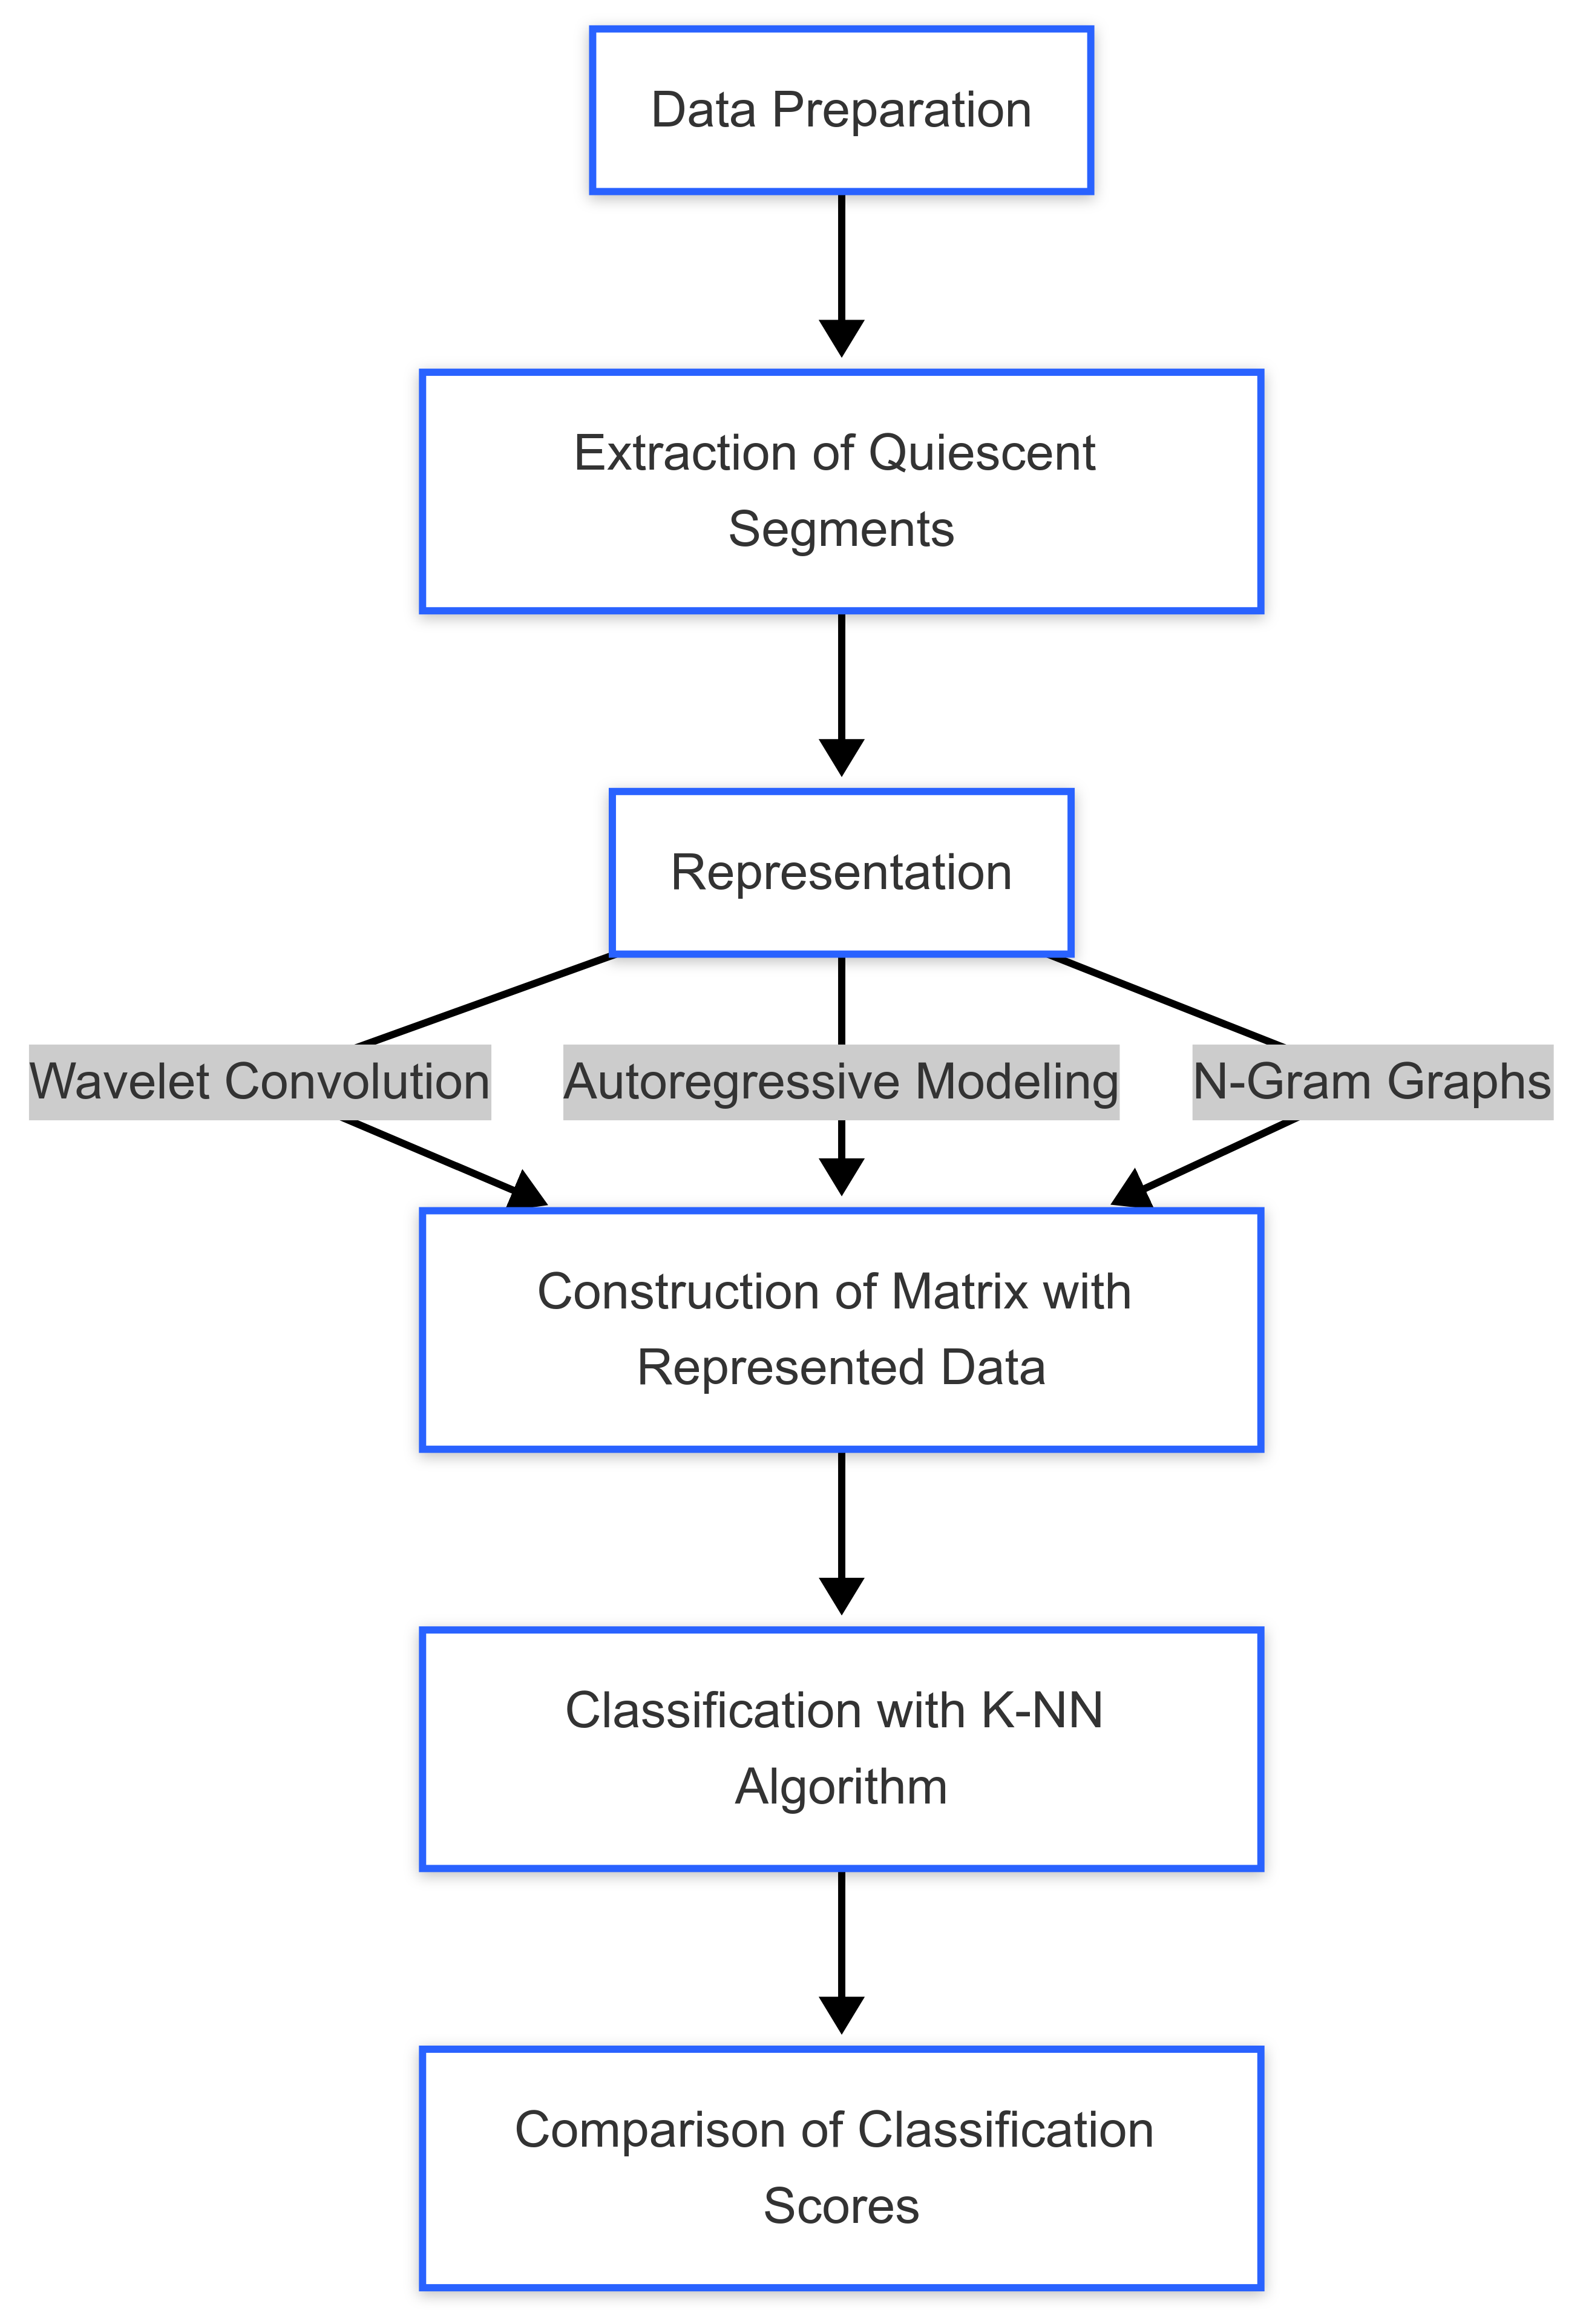
\includegraphics[width=0.9\linewidth]{PIPES.png}
	\caption{The processing pipeline consists of sequential stages, beginning with data preparation, followed by the extraction of quiescent segments from each stage in the transition to epilepsy. The raw signals of each quiescent segment are then transformed into the selected representations. Each representation is followingly used to construct a corresponding feature matrix, which serves as input for classification using the k-Nearest Neighbors (k-NN) algorithm. Finally, the classification scores with 10-fold cross validation are statistically compared.}
	\label{fig:pipeline}
\end{figure}

\section{Results}
The Friedman test revealed significant differences in classification accuracy across the three primary feature representation methods—Wavelets, Auto-Regressive, and N-Gram Graphs (\(
\chi^2 = 36.57, p < 0.001
\)).
To determine the relative performance of these methods, Bonferroni-corrected Wilcoxon rank-sum tests were conducted.

The Auto-Regressive representation consistently demonstrated superior accuracy compared to both Wavelet-based (\(
p = 0.0016
\))
and N-Gram Graph (\(
p = 0.0018
\))
representations. While Wavelets and N-Gram Graphs did not exhibit significant differences in accuracy (\(
p = 1.0
\)),
the N-Gram Graph approach showed a trend toward higher performance compared to the Wavelet-based method.

The baseline classifiers (Dummy and Basic) performed at chance level and remained consistently inferior to the three primary representations. Both the Auto-Regressive and N-Gram Graph methods significantly outperformed these baselines, while Wavelets showed no significant advantage over Basic features in accuracy (\(
p = 0.073
\)).

\begin{figure}[htbp]
    \centering
    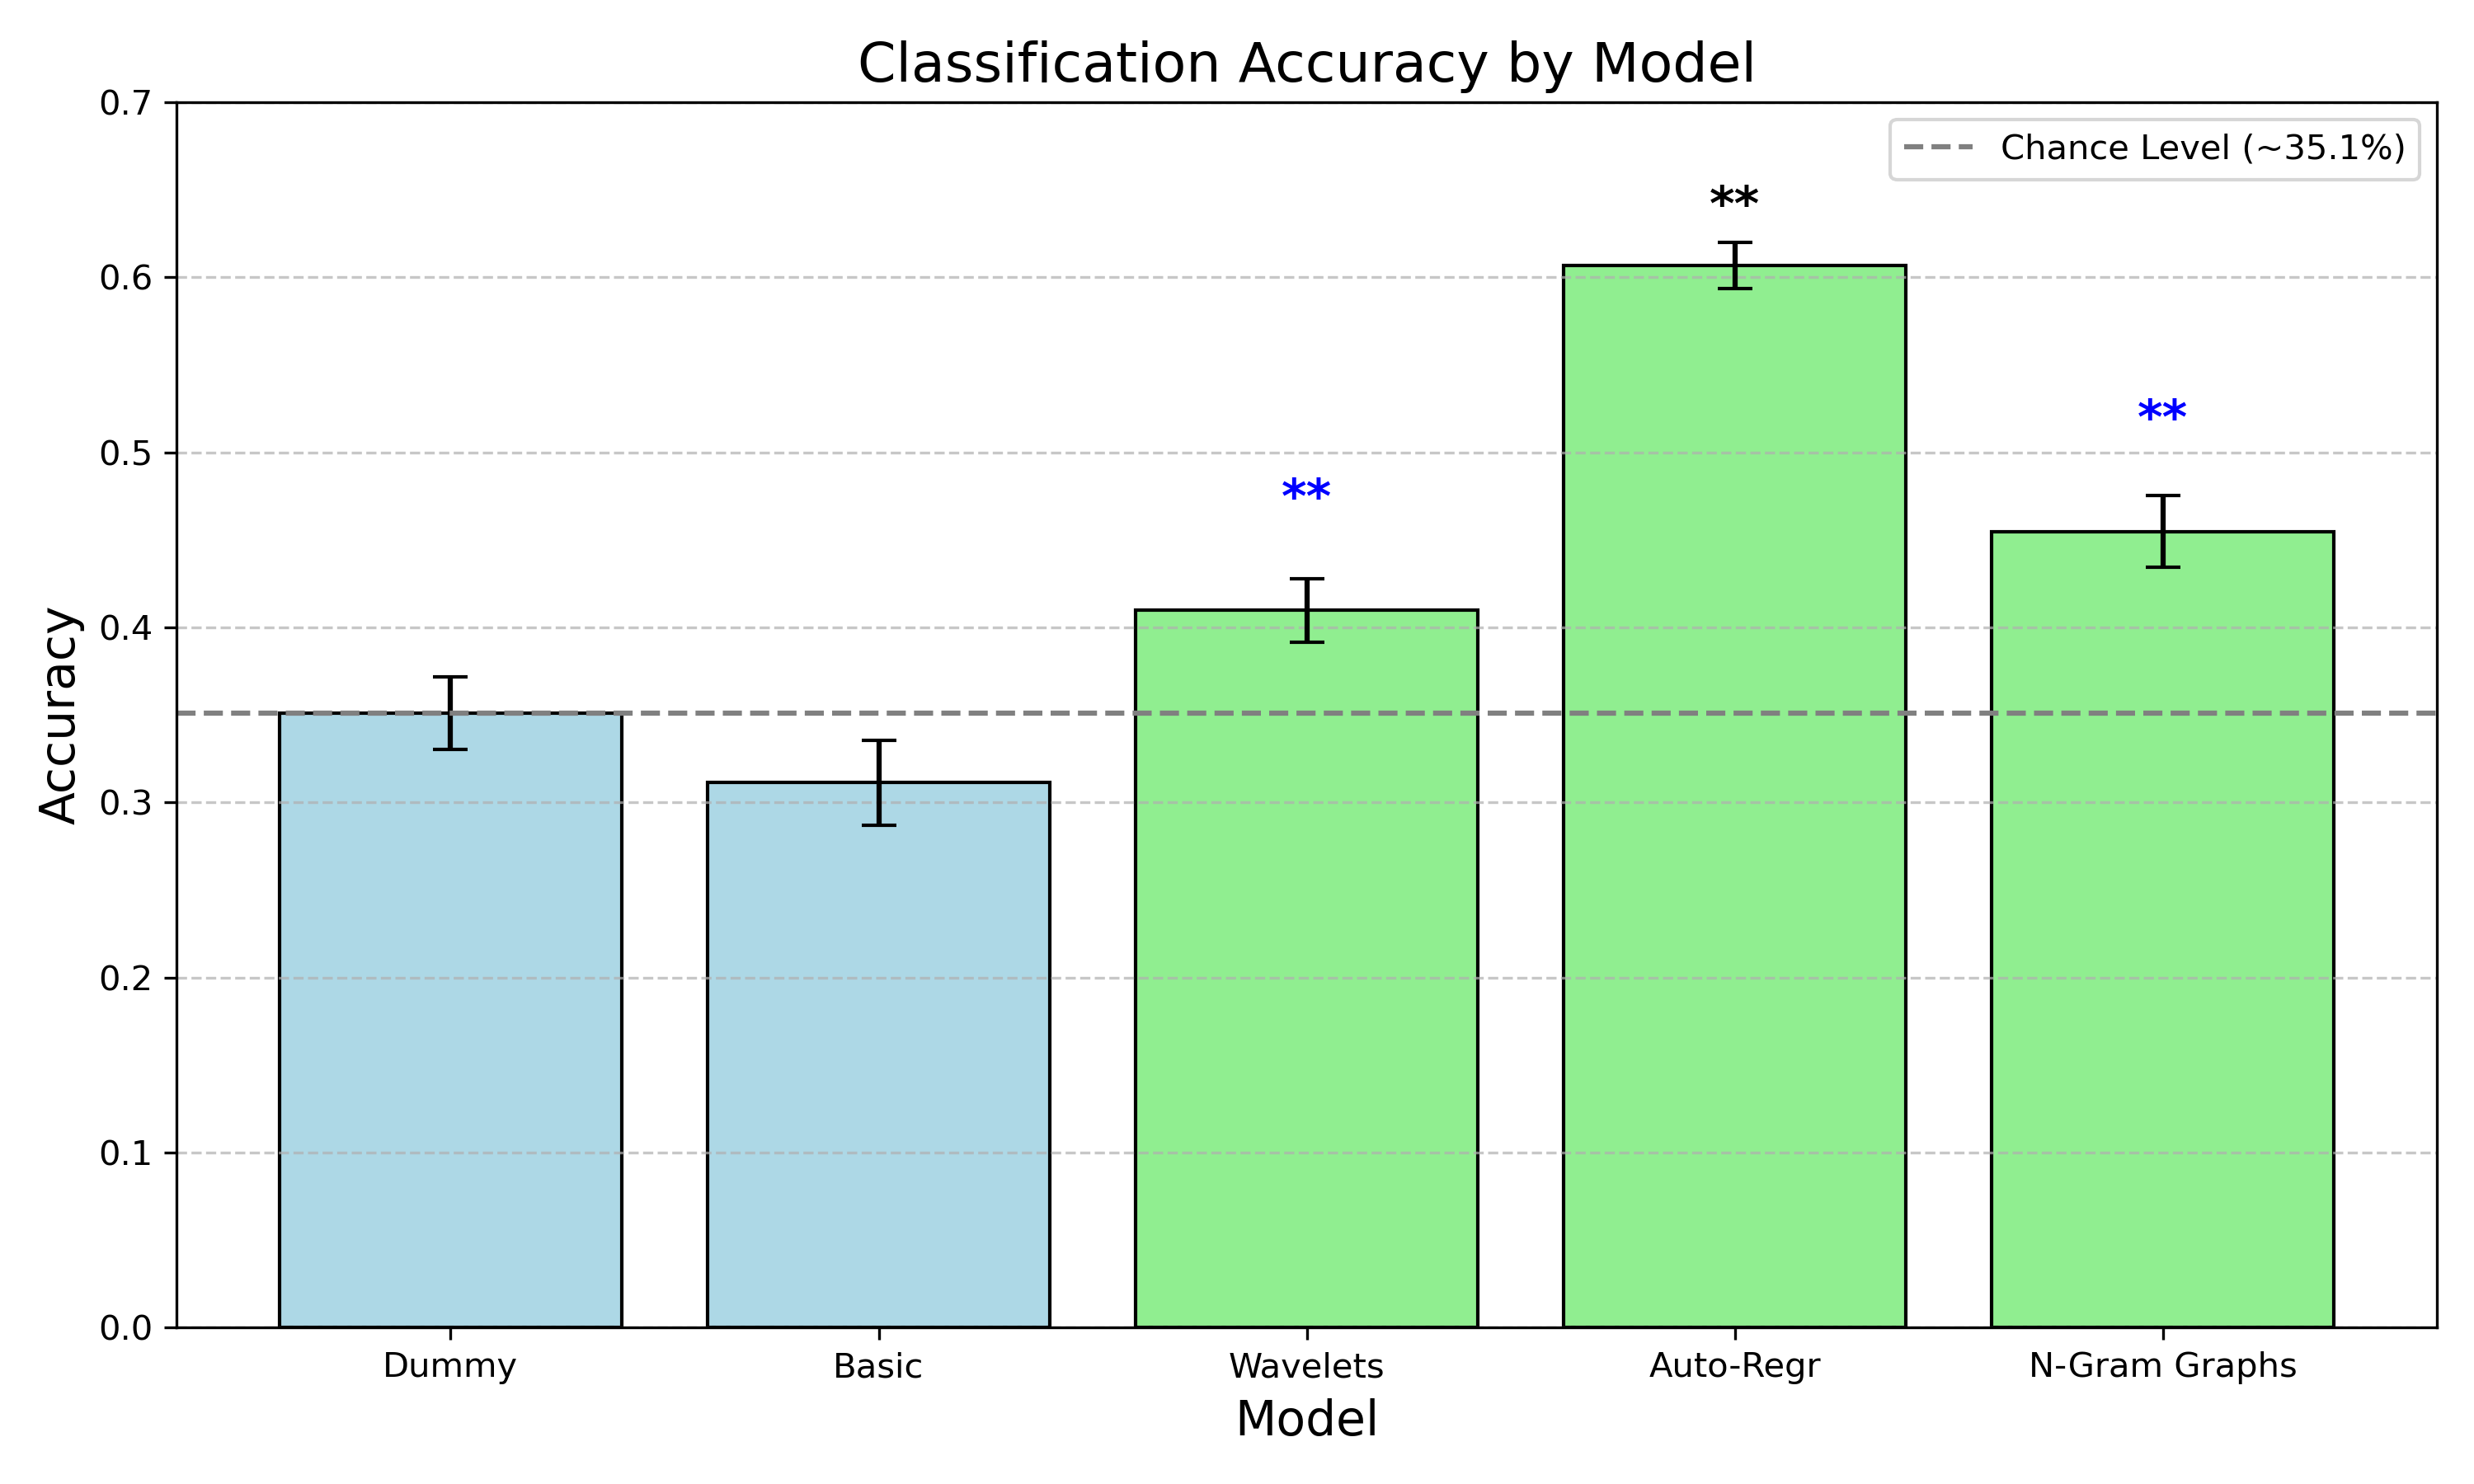
\includegraphics[width=\linewidth]{barplot_accuracies.png}
    \caption{\textcolor{red}{Classification accuracy by model for quiescent segment classification in different states of epilepsy. Bars indicate mean accuracy across 10-fold cross-validation, with error bars showing the standard error of the mean (SEM). The dashed gray line denotes chance-level performance, computed as the proportion of the most frequent class (Endogenous), approximately 35.1\%. Asterisks above the bars indicate statistically significant improvements compared to the baseline "Dummy" classifier, based on Bonferroni-corrected Wilcoxon rank-sum tests (*$p < .05$, **$p < .01$, ***$p < .001$). Auto-regressive modeling ("Auto-Regr") significantly outperforms all other models, achieving an accuracy of over 60\%. While this performance is substantially above chance and suggests the presence of discriminative signal features, it still reflects moderate classification difficulty given the nature of the data and task.}}
    \label{fig:accuracies}
\end{figure}

\subsection*{F1-Macro Score Comparisons}
The Friedman test for F1-macro scores also indicated significant performance differences among the feature representation methods (\(
\chi^2 = 35.44, p < 0.001
\)).
Pairwise comparisons confirmed that the Auto-Regressive representation produced significantly higher F1-macro scores than both Wavelets (\(
p = 0.0016
\))
and N-Gram Graphs (\(
p = 0.0029
\)).
No significant difference was observed between Wavelets and N-Gram Graphs in terms of F1-macro scores (\(
p = 0.963
\)),
mirroring the accuracy results.

Once again, the baseline classifiers were outperformed by all three primary methods. While Basic features exhibited marginally better performance than the Dummy classifier, their F1-macro scores remained significantly lower than those achieved by Auto-Regressive and N-Gram Graph-based representations.

\begin{figure}[htbp]
	\centering
	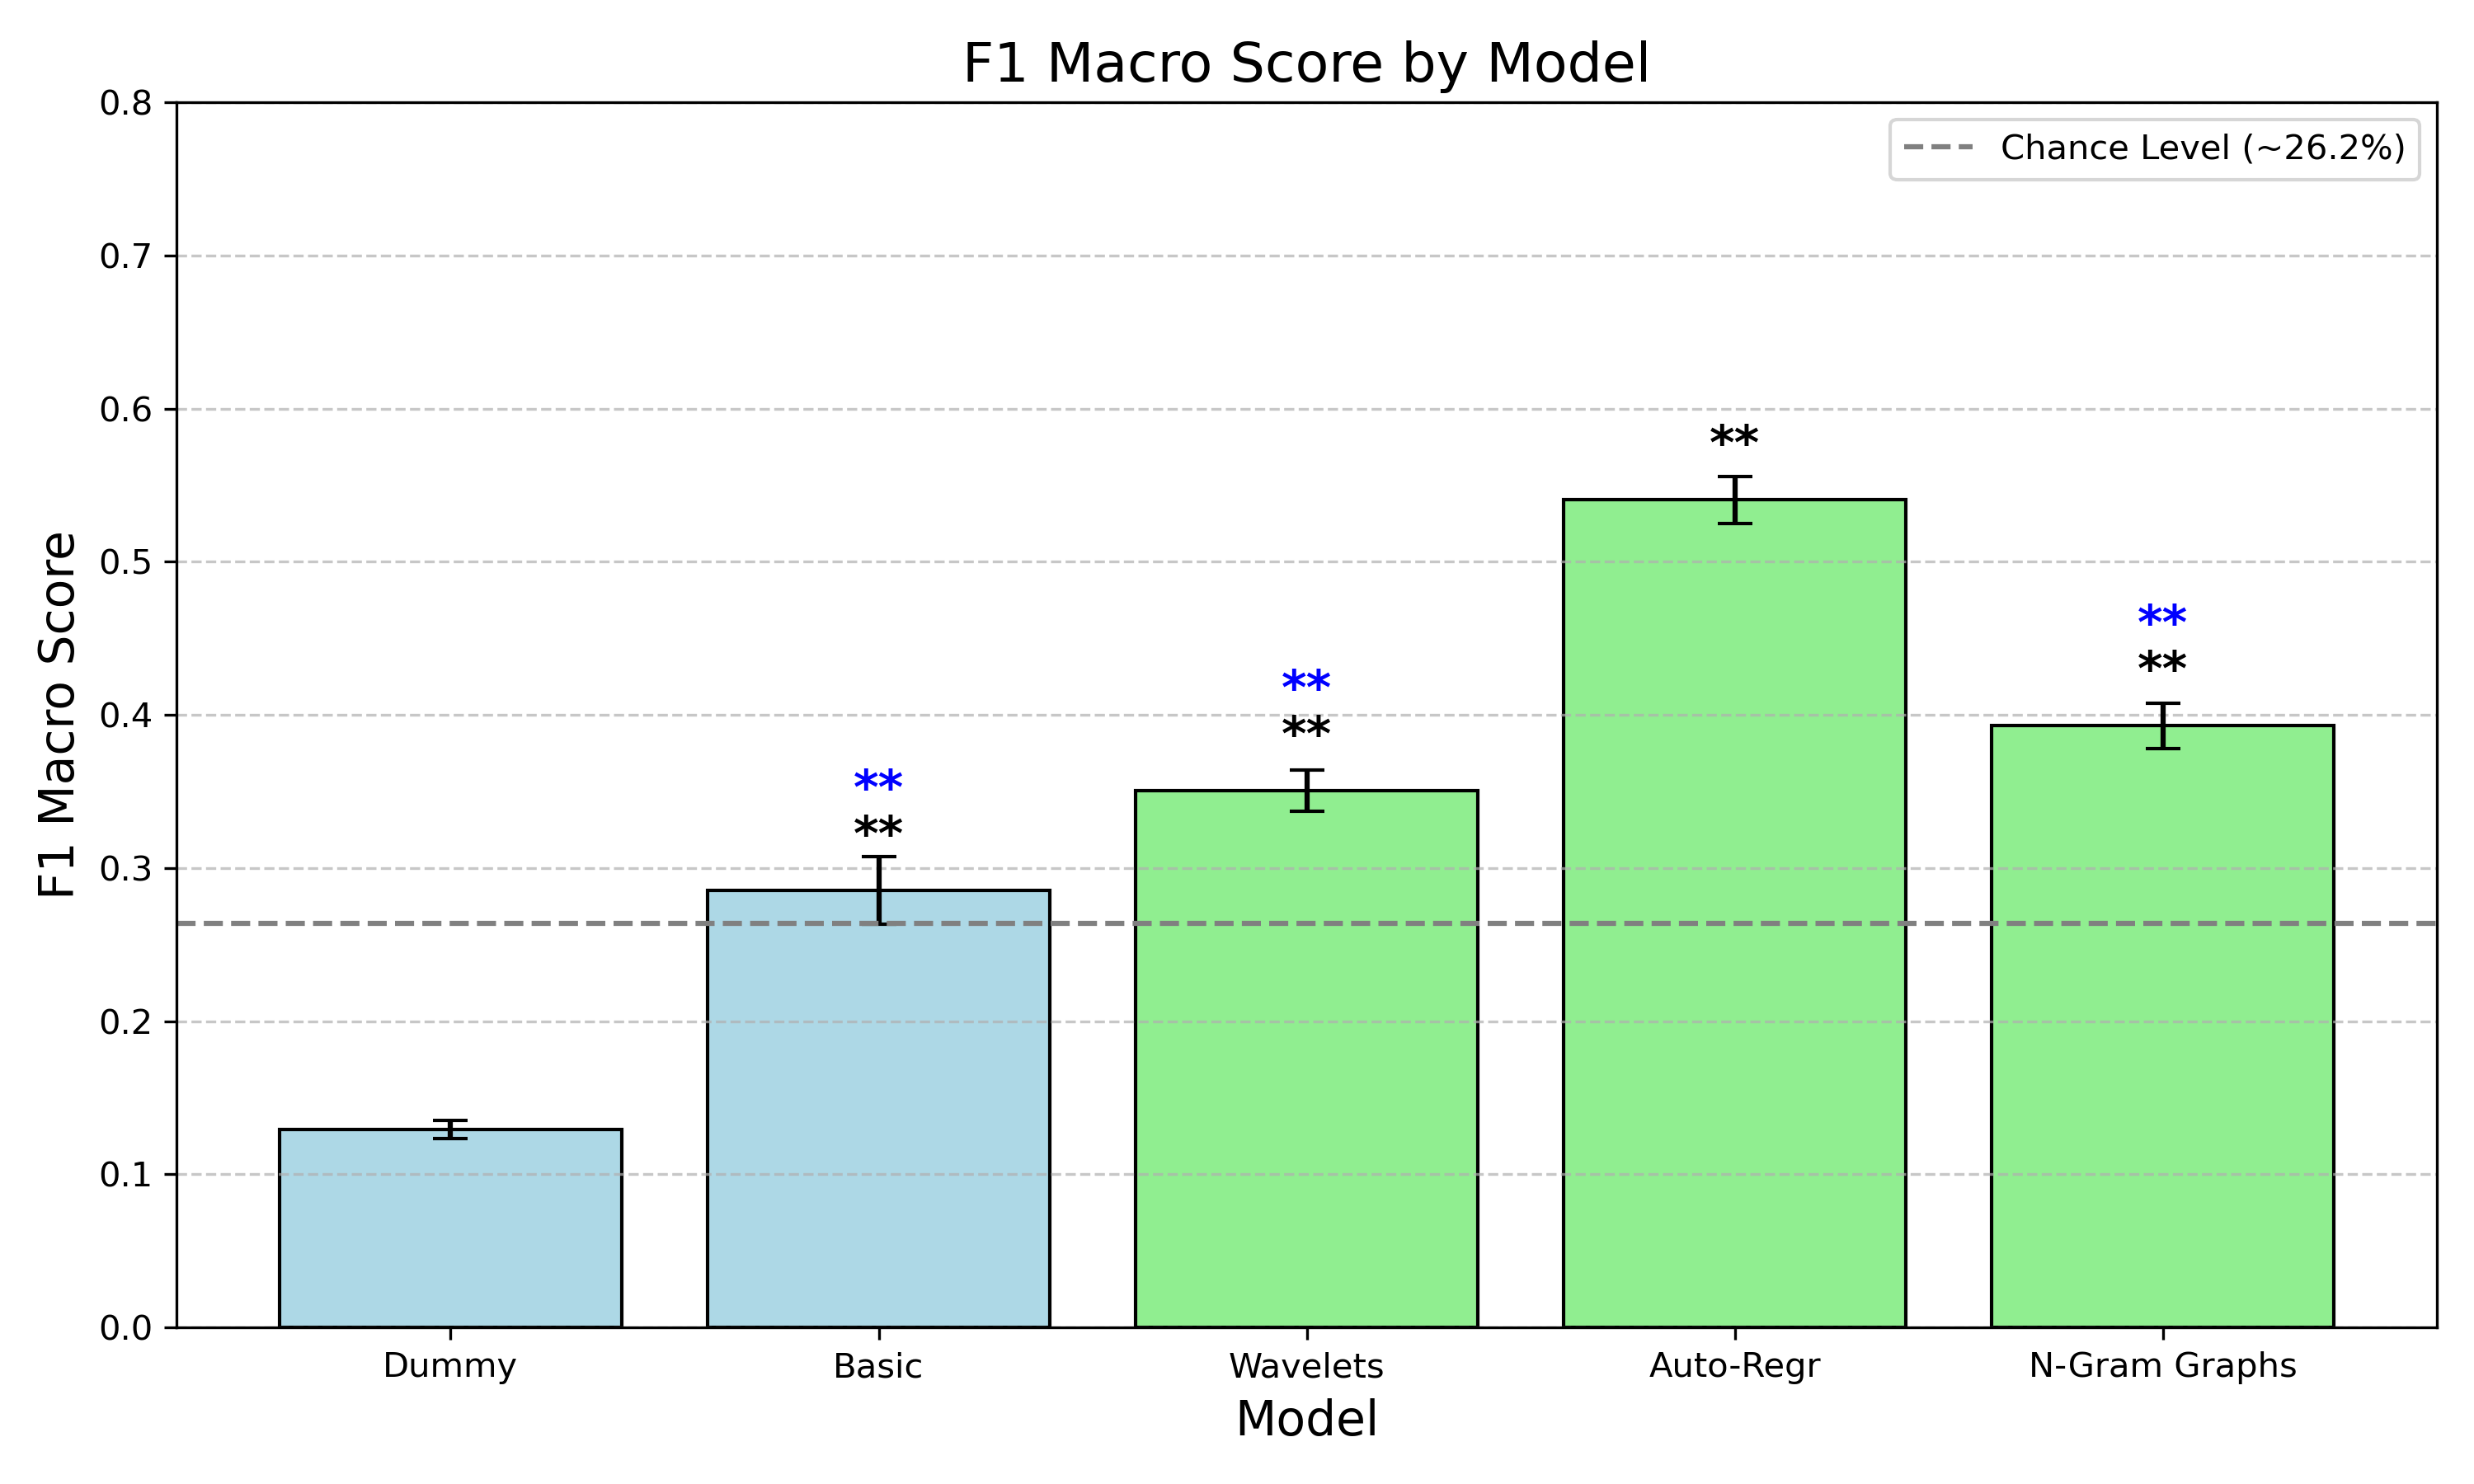
\includegraphics[width=\linewidth]{barplot_f1_macro.png}
	\caption{%
		\textcolor{red}{F1 macro scores achieved by each model for classifying quiescent segments across different epileptic states. Bars indicate mean F1 macro scores over 10-fold cross-validation, with error bars representing the standard error of the mean (SEM). The dashed gray line marks the estimated chance-level F1 macro score ($\sim$26.2\%), computed based on class imbalance. Asterisks above bars indicate statistically significant improvements over the "Dummy" baseline (*$p < .05$, **$p < .01$, ***$p < .001$), while blue asterisks highlight significant differences relative to the "Auto-Regr" model. Among the models, "Auto-Regr" achieves the highest F1 macro score ($>0.55$), suggesting that it captures discriminative temporal patterns in the quiescent signal segments. Although this performance level indicates meaningful structure in the data, it also reflects the inherent difficulty of the task, which involves subtle distinctions between relatively similar signal segments.}%
	}
	\label{fig:f1macro}
	\end{figure}

Across both classification accuracy and F1 macro scores, the Auto-Regressive representation consistently demonstrated the highest performance, significantly outperforming the Wavelet and N-Gram Graph-based approaches \textcolor{red}{(see Figures~\ref{fig:accuracies} and~\ref{fig:f1macro})}. The latter two methods exhibited comparable results, with no statistically significant differences between them. The baseline classifiers, were consistently inferior to the three primary feature representations. These results highlight the effectiveness of Auto-Regressive features in capturing relevant information for classification, while both Wavelet and N-Gram Graph methods provide alternative yet less optimal representations.

\section{Discussion - Future Directions}

The purpose of this thesis was twofold. Firstly, to determine which representation of the data would uncover the most informative characteristics {\textcolor{red}{for distinguishing quiescent segments across different stages of epileptogenesis} and consequently to examine the nature and distinguishability of these periods of quiescence. Starting from the latter, the ability of our classification pipeline to differentiate between quiescense as part of the endogenous network activity, in contrast to quiescence during the phase of transition to epilepsy, or during its complete onset, indicates that there are marked differences between these ostensibly facsimile signals. Quiescence during endogenous activity, or in our case before any experimental intervention, can be synonymous with Down-states, which are alternating with Up (active) states giving rise to the bistable phenomenon of slow-oscillations (SOs), which can be characterized as the default cortical activity, since they are observed even in the complete absence of external inputs to the cortex \cite{sanchez2017}. SOs were thought to arise solely due to intrinsic adaptive properties of neurons, but evidence suggests that they are also a result of stochastic fluctuations \cite{jercog2017}. The rythmic alternation of up states and down states indicate a cyclical functional dynamic of the cortex, which in vivo is observed during sleep or states of reduced arousal.

However, as the balance of the system is perturbed and the transition to epilepsy is initiated, periods of quiescence are not defined by the same electrical and functional parameters as down states. This suggests that while down states are a specific type of quiescent state, not all quiescent periods can be classified as down states.  Quiescence in epileptic transitions may reflect network instability preceding seizure onset. This aligns with observations that critical slowing down (CSD)— a phenomenon where a dynamical system approaching a critical transition takes longer to recover from small perturbations—can serve as a biomarker for seizure susceptibility \cite{maturana2020} and in particular, quiescent segments could correspond to markers of CSD. Additionally, evidence from Sheybani et al. (2023) \cite{sheybani2023} suggests that periods of low-frequency oscillations interrupt normal network function and correlate with cognitive impairments, further supporting the idea that quiescent states could potentially play an active role in epilepsy pathophysiology.

The fact that during down states neuronal activity continues albeit reduced \cite{reig2010}, which could potentially provide us with valuable network information in conjunction with the aforementioned lines of evidence should motivate more extensive research into the elucidation of their complete neurophysiological and functional profile. This thesis was an attempt to contribute towards this direction.

That being said, the careful examination of quiescent segments during the transition to epilepsy depends heavily on the way that useful information are extracted from the original signal. Among the different feature representation methods tested in this study, autoregressive modeling demonstrated the highest classification performance. This is particularly notable given that autoregressive models operate in the time domain, unlike wavelets, which examine the time-frequency domain, and N-Gram Graphs, which analyze statistical co-occurrences of local patterns. The advantage of autoregressive modeling in this context suggests that preserving the intrinsic temporal structure of the signal is crucial for differentiating quiescent states in epilepsy. This could indicate that the transition to epilepsy is not marked by abrupt spectral shifts, which would be highlighted by a superiority of the wavelet method, but by gradual alterations in synaptic and network dynamics. Both convolution with morlet wavelets, which are extensively used in neuroscience and n-gram graphs, which in this particular experiment showed promising results, should be considered and adapted for appropriate analyses of LFP signals, with autoregressive modeling being the most appropriate choice in this context, possibly due to its ability to capture transient phenomena.

\subsection{Future Directions}

The current study focuses on classifying quiescent periods in induced epileptic activity. While this provides a controlled framework for assessing network dynamics during epileptogenesis, future research should investigate whether similar classification success can be achieved in models of spontaneous epilepsy or in human recordings. Such an extension would allow for the differentiation between universal markers of epileptogenesis and model-specific features. If quiescent states during induced seizures exhibit similar differentiability in naturally occurring epilepsy, this would strengthen the argument that these periods encode meaningful information about the transition to pathological brain states.

Given the demonstrated effectiveness of autoregressive modeling in distinguishing quiescent states, future work could explore hybrid feature representations that integrate time-domain information with complementary perspectives, such as spectral features from wavelet analysis or more advanced models. Crucially, future work could involve a more exhaustive search for optimal parameters across the three primary feature representations. While our study employed reasonable parameter settings based on existing literature and practical constraints, it is possible that a more complete search, would lead to optimized performance.

\newpage

\printbibliography
\end{document}


